\documentclass[english,course]{Notes}

\title{Algebraic stacks}
\subject{Algebraic geometry}
\author{Stefano Maggiolo}
\email{s.maggiolo@gmail.com}
\speaker{Barbara Fantechi}
\date{12}{01}{2009}
\dateend{12}{01}{2009}
\place{SISSA, Trieste}

\newcommand{\defcat}[6]{
  #1 ≔ \left\{
  \begin{array}{l}
    #2 ∈ \Obj(#1) \quad ⇔ \quad #4\\
    #5 ∈ \Mor(#2, #3) \quad ⇔ \quad #6
  \end{array}
  \right.
}

\newcommand{\defcatold}[6]{
  #1 ≔ \left\{
  \begin{array}{ll}
    \Obj(#1)\colon & \left\{#2 \middle| #4 \right\}\\
    \Mor(#2, #3)\colon & \left\{#5 \middle| #6 \right\}
  \end{array}
  \right.
}


\begin{document}

\section{Introduzione}\lecture[2 ore]{12}{01}{2009}

\begin{example}
  Siano $V$ uno spazio vettoriale di dimensione finita su un campo algebricamente chiuso $K$ e $r ≤ \dim V$; possiamo considerare la grassmanniana dei sottospazi vettoriali di $V$ di dimensione $r$. Questo spazio viene descritto come insieme, ma ha una naturale descrizione come varietà algebrica. Inoltre è uno \emph{spazio di moduli fine\/}:
  \begin{itemize}
    \item la varietà d'incidenza $Γ(r, V) ≔ \{(W, x) \mid W ∈ G(r, V) ∧ v ∈ W\}$ è un sottofibrato di rango $r$ del fibrato banale $G(r, V) × V$ su $G(r, V)$;
    \item se $X$ è uno schema ed $E ⊆ X × V$ è un sottofibrato di rango $r$, allora esiste unica $φ_E\colon X → G(r, V)$ tale che $E = φ_E^⋆(Γ(r, V))$, cioè il diagramma
      \[
      \begin{tikzpicture}
        \def\x{1.5}
        \def\y{-1.2}
        \node (A0_0) at (0*\x, 0*\y) {$E$};
        \node (A0_1) at (1*\x, 0*\y) {$Γ(r, V)$};
        \node (A1_0) at (0*\x, 1*\y) {$X$};
        \node (A1_1) at (1*\x, 1*\y) {$G(r, V)$};
        \path (A0_0) edge [->] node [auto] {$\scriptstyle{}$} (A0_1);
        \path (A0_0) edge [->] node [auto] {$\scriptstyle{}$} (A1_0);
        \path (A0_1) edge [->] node [auto] {$\scriptstyle{}$} (A1_1);
        \path (A1_0) edge [->] node [auto,swap] {$\scriptstyle{φ_E}$} (A1_1);
      \end{tikzpicture}
      \]
      è cartesiano.
  \end{itemize}
\end{example}

\begin{exercise}
  Dimostrare che $G(r, V)$ è uno spazio di moduli fine.
\end{exercise}

\begin{remark}
  Come mappa di insiemi, $φ_E$ manda $x$ nel punto $[E_x]$ corrispondente al sottospazio vettoriale $E_x ⊆ \{x\} × V$.
\end{remark}
Assumendo sempre $r$ e $V$ fissi, consideriamo un'altra interpretazione. Sia $γ\colon \Schemes^\opp{} → \Sets$ il funtore controvariante definito in questo modo:
\begin{itemize}
  \item se $X$ è uno schema, \[ γ(X) ≔ \{E → X \mid \text{$E$ sottofibrato di rango $r$ di $X × V$}\}\text{;}\]
  \item se $ψ\colon X → Y$ è un morfismo e $E_Y ⊆ Y × V$ è un sottofibrato di rango $r$, \[ γ(ψ)(E_Y) ≔ ψ^⋆(E_Y) = {(ψ × \id)}^{-1}(E_Y)\text{.}\]
\end{itemize}
Con questo linguaggio, il fatto che $G(r, V)$ è uno spazio di moduli fine si esprime dicendo che $γ$ è naturalmente isomorfo al funtore di Yoneda $\ho_{G(r, V)}$. In particolare, a $\id ∈ \Aut(G(r, V))$ corrisponde il fibrato $Γ(r, V) → G(r, V)$.

\begin{example}
  Se $X$ è una varietà proiettiva (volendo anche liscia), consideriamo $\Pic(X)$, l'insieme dei fibrati lineari su $X$ modulo isomorfismo; $\Pic(X)$ ha una struttura di spazio topologico con, in generale, infinite componenti connesse e ogni componente ha una struttura di varietà algebrica. Inoltre, la struttura di gruppo su $\Pic(X)$ (data dal prodotto tensore) è compatibile con la struttura di varietà algebrica. Grazie a questo si dimostra che tutte le componenti connesse sono isomorfe tra loro e quindi si può considerare solamente la componente connessa dell'identità, $\Pic^0(X)$.
\end{example}

Come costruire il funtore corrispondente a $\Pic^0(X)$, per ottenere una situazione analoga alla precedente?

\begin{definition}
  Sia $X$ una varietà proiettiva liscia; si definisce il funtore controvariante $π\colon \Schemes^\opp{} → \Sets$ mediante:
  \begin{itemize}
    \item se $S$ è uno schema, \[ π(S) ≔ \{ L \mid \text{$L$ fibrato lineare su $X × S$}\} / ∼\text{,}\] dove $L ∼ L′$ sono equivalenti se e solo se esiste $M ∈ \Pic(S)$ tale che $L′ ≅ L ⊗ p_S^⋆ M$, dove $p_S\colon X × S → S$ è la proiezione\footnote{In tal modo, $L′_{|X × \{s\}} ≅ L_{|X × \{s\}} ⊗ p_S^⋆ M_{|X × \{s\}} = L_{|X × \{s\}}$, cioè si considerano equivalenti due fibrati se si restringono sulla fibra allo stesso oggetto.};
    \item se $φ\colon S′ → S$ e $L ∈ \Pic(X × S)$, \[ π(φ)(L) ≔ φ^⋆ L\text{;}\] si può verificare che questo passa alla relazione d'equivalenza.
  \end{itemize}
\end{definition}

Non dimostreremo il seguente teorema.

\begin{theorem}
  Esiste unica una struttura di varietà algebrica (con infinite componenti connesse) su $\Pic(X)$ ed esiste un fibrato lineare $ℒ$, detto \emph{fibrato di Poincaré\/} su $X × \Pic(X)$ tale che $π → \ho_{\Pic(X)}$ è una equivalenza naturale e $ℒ$ corrisponde a $\id ∈ \Aut(\Pic(X))$; inoltre $ℒ$ è unico a meno di pullback tramite la proiezione $X × \Pic(X) → \Pic(X)$.
\end{theorem}

Possiamo riformulare il teorema nel modo seguente. Il funtore $π$ è rappresentato da una varietà algebrica liscia (con infinite componenti connesse); da questo segue che i $K$-punti di $\Pic(X)$, per definizione in corrispondenza biunivoca con $\Mor(\Spec K, \Pic(X))$, per la rappresentabilità sono in corrispondenza biunivoca anche con $π(\Spec K)$; questo però corrisponde a $\Pic(X)$, a priori a meno di pullback di fibrati lineari sul punto, che però sono solo banali.

Perché abbiamo la complicazione della tensorizzazione per un pullback? Questo viene dal fatto che due fibrati lineari possono avere diversi modi per essere isomorfi, cioè dal fatto che, al contrario dei sottospazi vettoriali di $V$, un fibrato lineare può avere un gruppo di automorfismi non banali.

La prima apparizione degli stack è all'inizio degli anni '60, in francese, con il nome di \emph{champs}, da parte di Giraud, studente di Grothendieck. Ma l'introduzione degli stack come oggetti geometrici è dovuta a Deligne e Mumford, alla fine degli anni '60, quando si posero il seguente problema.

\begin{problem}
  Sia $g ≥ 2$ un intero; si vuole dare una struttura di varietà algebrica a $M_g$, lo spazio delle curve lisce proiettive di genere $g$ modulo isomorfismo; se possibile come spazio di moduli fine (cioè in modo che sia la rappresentazione di un funtore adatto).
\end{problem}

Perché di genere maggiore o uguale a $2$? Perché le curve con tali proprietà e di genere $0$ sono solo $ℙ^1$, mentre quelle di genere $1$ sono curve ellittiche, studiate da molto tempo e sufficientemente comprese. Il primo approccio a questo problema è proprio di Riemann, che dimostrò che per descrivere una curva di genere $g$ sono necessari $3g-3$ parametri che chiamò \emph{moduli}.

\begin{example}
  Le curve di genere $2$ sono tutte iperellittiche; in particolare, se $C$ ha genere $2$ esiste un unica mappa $C → ℙ^1$ due a uno, che è ramificata in $6$ punti. Viceversa, un tale morfismo ramificato determina una curva di genere $2$. Quindi le curve di genere $2$ sono in corrispondenza con i sottoinsiemi di $6$ punti di $ℙ^1$ modulo automorfismi di $ℙ^1$; se questi punti fossero ordinati, si potrebbero esaurire gli automorfismi fissando $p_1 = 0$, $p_2 = 1$, $p_3 = ∞$ e il quoziente avrebbe dimensione $3$. Non essendo ordinati, c'è un'altra azione di $S_6$ da tenere in considerazione, che però non cambia la dimensione del quoziente.
\end{example}

\begin{example}
  In genere $3$, abbiamo le curve iperellittiche (con morfismo su $ℙ^1$ ramificato in $8$ punti) e le curve non iperellittiche, che ammettono un unico morfismo su $ℙ^2$ (modulo automorfismo di $ℙ^2$) su una curva di grado $4$. Le prime hanno $5$ moduli, calcolati nel modo visto prima; di conseguenza le seconde devono averne $6$.
\end{example}

\begin{exercise}
  Dimostrare che le curve di genere $3$ non iperellittiche hanno $6$ moduli.
\end{exercise}

%\begin{proof}[Soluzione.]
%  Le quartiche lisce di $ℙ^2$ sono tutte curve di genere $\binom{4-1}{2} = 3$ per la formula del genere. La varietà delle quartiche di $ℙ^2$ ha dimensione $\binom{4+2}{4}-1 = 14$; gli automorfismi di $ℙ^2$ sono $ℙ\GL(3)$, di dimensione $8$; dobbiamo quindi dimostrare che, per la generica quartica $C$, $\Aut(C) / G$ è un gruppo finito, dove $G$ è il gruppo degli automorfismi di $C$ indotto da $ℙ\GL(3)$. 
%\end{proof}

\begin{definition}
  Sia $μ_g\colon \Schemes^\opp{} → \Sets$ il funtore definito in questo modo:
  \begin{itemize}
    \item dato uno schema $S$, \[ μ_g(S) ≔ \Biggl\{p\colon C → S \Biggm| \parbox{4cm}{$p$ liscio, proiettivo, con $C_s ≔ p^{-1}(s)$ una curva di genere $g$ per ogni $s ∈ S$}\Biggr\} \Biggm/ ∼\text{,}\] dove $p ∼ p′$ se esiste un diagramma di questo tipo:
      \[
      \begin{tikzpicture}
        \def\x{1.5}
        \def\y{-1.2}
        \node (A0_0) at (0*\x, 0*\y) {$C$};
        \node (A0_1) at (1*\x, 0*\y) {$C′$};
        \node (A1_0) at (0*\x, 1*\y) {$S$};
        \node (A1_1) at (1*\x, 1*\y) {$S′$.};
        \path (A0_0) edge [->] node [auto] {$\scriptstyle{}$} node [sloped] {$\scriptstyle{\widetilde{\ \ \ }}$} (A0_1);
        \path (A1_0) edge [-,double] node [auto] {$\scriptstyle{}$} (A1_1);
        \path (A0_1) edge [->] node [auto] {$\scriptstyle{p′}$} (A1_1);
        \path (A0_0) edge [->] node [auto,swap] {$\scriptstyle{p}$} (A1_0);
      \end{tikzpicture}
      \]
    \item dato un morfismo $φ\colon S′ → S$ e una famiglia $p\colon C → S$, \[ μ_g(φ)(p)\colon C ×_S S′ → S′\text{;}\] questa nuova famiglia mantiene tutte le proprietà richieste.
  \end{itemize}
\end{definition}

In particolare, osserviamo che $μ_g(\Spec K) = M_g$.

\begin{problem}
  Esiste una struttura di varietà algebrica su $M_g$ tale che $μ_g$ e $\ho_{M_g}$ siano naturalmente equivalenti? In altre parole, $μ_g$ è rappresentabile?
\end{problem}

La risposta a questa domanda è nella seguente proposizione, che verrà dimostrata in seguito.

\begin{proposition}
  Se si definisce $μ_g^0$ come $μ_g$, con la condizione aggiuntiva che ogni fibra sia una curva rigida (senza automorfismi non banali), allora $μ_g^0$ è rappresentabile con una varietà liscia $M_g^0$, quasi proiettiva, connessa, di dimensione $3g-3$, a meno che $g = 2$ (perché tutte le curve di genere $2$, essendo iperellittiche, hanno almeno un'involuzione).
\end{proposition}

\begin{example}
  Per $g = 3$, si considera $U$, l'insieme delle quartiche di $ℙ^2$ lisce e rigide (cioè, i cui soli automorfismi siano indotti da automorfismi di $ℙ^2$); allora $U / ℙ\GL(3, K)$ è $M_3^0$, dato che l'azione di $ℙ\GL(3, K)$ è senza punti fissi. Com'è descritta la curva universale? Sia $Γ_U ⊆ U × ℙ^2$ la varietà d'incidenza, con punti $(C, x)$ con $x ∈ C$; allora $Γ_U / ℙ\GL(3, K) → U / ℙ\GL(3, K)$ è la famiglia universale, in quanto le sue fibre sono esattamente le fibre di $Γ_U → U$. Se si cerca di inserire anche le quartiche non rigide, nel quozientare si incontrano problemi a causa degli stabilizzatori non banali.
\end{example}

Come si dimostra che un funtore non è rappresentabile? Vediamo un'esempio di dimostrazione per il funtore $μ_g$.

\begin{proposition}
  Il funtore $μ_g$ non è rappresentabile.
\end{proposition}

\begin{proof}
  Abbiamo visto che i problemi nascono dalle curve con automorfismi; sia quindi $C_0$ una curva liscia di genere $g$ con un automorfismo $φ$ diverso dall'identità. Per fissare le idee, supponiamo $φ^2 = \id$ (in realtà è sempre possibile trovare una curva con un'involuzione, dato che in ogni genere ci sono curve iperellittiche). Consideriamo $S ≔ 𝔸^1 ∖ \{0\}$ e la famiglia banale $p\colon C_0 × S → S$; $p$ è il pullback di $C_0 → \Spec K$ via l'unica mappa $S → \Spec K$. Se $μ_g$ fosse rappresentabile, $p$ dovrebbe necessariamente corrispondere a un morfismo costante $S → M_g$.
  
  Siano ora $α\colon S → S$ l'involuzione data da $α(t) ≔ -t$ e $S′ ≔ S / α$, ancora isomorfo a $S$ con coordinata $s ≔ t^2$. Sia inoltre $C′ ≔ (C_0 × S) / (φ, α)$, dove $(φ, α)(x,t) = (φ(x), -t)$. Quindi il morfismo $p$ induce un morfismo $p′\colon C′ → S′$, con le stesse fibre; in particolare si dimostra che $C_0 × S ≅ C′ ×_{S′} S$. Allora tutte le fibre di $p′$ sono isomorfe a $C_0$, perciò se il funtore fosse rappresentabile, $p′$ dovrebbe essere il pullback di una famiglia universale su $M_g$ tramite una mappa costante, e $C′$ dovrebbe essere un prodotto, ma non è così.∎
\end{proof}

In questo caso, si dice che $C′ → S′$ è una famiglia \emph{isotriviale}, cioè tutte le fibre sono isomorfe ma globalmente non è un prodotto. 

\begin{proof}[Dimostrazione alternativa.]
  Sia $T ≔ 𝔸^1$ e consideriamo $C″ ≔ (C_0 × T)/∼$ dove $(x, t) ∼ (x′, t′)$ se sono uguali o $x′ = φ(x)$ e $\{t, t′\} = \{-1, 1\}$. In altre parole, si identificano le fibre su $-1$ e $1$ e si incollano rovesciate tramite $φ$. Si dimostra che $C″$ ha una struttura di varietà algebrica.
  
  Sia ora $T″ ≔ T / (-1=+1)$; $T″$ si realizza in $𝔸^2$ tramite una cubica nodata. Ancora, $C″ → T″$ è una famiglia isotriviale.∎
\end{proof}

\begin{exercise}
  Dimostrare che $C′$ non è un prodotto; si può assumere che $\Aut(C_0) ≅ \{\id, α\}$.
\end{exercise}

Il problema si pone allo stesso modo con i fibrati: tutti i fibrati dello stesso rango sono localmente isomorfi, ma questo non si estende in generale a un isomorfismo globale; per avere uno spazio di moduli fine, ovvero se si vuole considerare un fibrato come un morfismo in un qualche spazio, bisogna anche considerare gli isomorfismi dei morfismi, che nel caso della topologia sono le omotopie.

Cos'è andato storto nella definizione di $μ_g$? L'idea di uccidere tutti gli isomorfismi considerandoli tutti allo stesso modo. Se $μ_g$ fosse naturalmente isomorfo a $\ho_{M_g}$, allora $μ_g(S)$ sarebbe in b\^{i}ezione con $\Mor(S, M_g)$; per non dimenticare gli isomorfismi, si deve definire $μ_g(S)$ come un oggetto che ricordi sia un insieme di famiglie di curve di genere $g$ con le proprietà richieste, ma anche gli isomorfismi tra queste famiglie. Un oggetto tale è un \emph{gruppoide}, cioè una categoria in cui ogni morfismo è un isomorfismo.

\begin{example}
  Siano $ℭ$ e $ℭ′$ due categorie, $F, G\colon ℭ → ℭ′$ due funtori covarianti; un funtore manda oggetti in oggetti e morfismi in morfismi; se abbiamo una trasformazione naturale $ν\colon F → G$, questa manda un oggetto $x ∈ ℭ$ in un morfismo $ν(x)\colon F(x) → G(x)$, mentre manda un morfismo $f\colon x → y$ in un diagramma commutativo in $ℭ′$:
  \[
  \begin{tikzpicture}
    \def\x{1.5}
    \def\y{-1.2}
    \node (A0_0) at (0*\x, 0*\y) {$F(x)$};
    \node (A0_1) at (1*\x, 0*\y) {$G(x)$};
    \node (A1_0) at (0*\x, 1*\y) {$F(y)$};
    \node (A1_1) at (1*\x, 1*\y) {$G(y)$.};
    \path (A0_0) edge [->] node [auto] {$\scriptstyle{ν(x)}$} (A0_1);
    \path (A1_0) edge [->] node [auto,swap] {$\scriptstyle{ν(y)}$} (A1_1);
    \path (A0_1) edge [->] node [auto] {$\scriptstyle{G(f)}$} (A1_1);
    \path (A0_0) edge [->] node [auto,swap] {$\scriptstyle{F(f)}$} (A1_0);
  \end{tikzpicture}
  \]
  La trasformazione naturale $ν$ è un'equivalenza naturale se $ν(x)$ è un isomorfismo per ogni $x$. In particolare, se $ℭ′$ è un gruppoide, ogni trasformazione naturale $ν\colon F → G$ è un'equivalenza naturale.
\end{example}

\begin{corollary}
  I gruppoidi hanno una struttura di $2$-categoria, in cui ci sono:
  \begin{itemize}
    \item gli oggetti: i gruppoidi stessi;
    \item i morfismi: i funtori covarianti tra gruppoidi;
    \item i $2$-morfismi: le equivalenze naturali;
  \end{itemize}
  i $2$-morfismi, o morfismi tra morfismi, sono tutti invertibili; in particolare, se $X$ e $Y$ sono gruppoidi, allora $\Mor(X, Y)$, la categoria con oggetti i funtori e morfismi le trasformazioni naturali, è ancora un gruppoide.
\end{corollary}

L'idea è prendere la definizione di schema, scriverla in un modo in cui sia evidente che i morfismi formino un insieme, sostituire i gruppoidi agli insiemi e aggiustare le cose.

\begin{notation}
  Siano $ℭ$ e $ℭ′$ gruppoidi, $F, G\colon ℭ → ℭ′$ funtori, $ν$ una equivalenza naturale tra $F$ e $G$ (denotata $ν\colon F ⇒ G$); questa situazione è descritta dal seguente diagramma:
  \[
  \begin{tikzpicture}
    \def\x{1}
    \def\y{-1.2}
    \node (A0_0) at (0*\x, 0*\y) {$ℭ$};
    \node (A0_2) at (2*\x, 0*\y) {$ℭ′$};
    \path (A0_0) edge [->,bend left=30] node [auto] {$\scriptstyle{F}$} (A0_2);
    \path (A0_0) edge [->,bend right=30] node [auto,swap] {$\scriptstyle{G}$} (A0_2);
    \path (0.98*\x, -0.1*\y) -- (1.02*\x, 0.1*\y) 
      node [pos=0.5,sloped] {$\Longrightarrow$}
      node [pos=-0.4,auto,sloped] {$\scriptstyle{ν}$};
  \end{tikzpicture}
  \]
  si dice che il diagramma è $2$-commutativo.
\end{notation}

\begin{exercise}
  Costruire la composizione
  \[
  \begin{tikzpicture}[baseline]
    \def\x{1}
    \def\y{-1.2}
    \node (A0_0) at (0*\x, 0*\y) {$ℭ$};
    \node (A0_2) at (2*\x, 0*\y) {$ℭ′$};
    \node (A0_4) at (4*\x, 0*\y) {$ℭ″$};
    \path (A0_0) edge [->,bend left=30] node [auto] {$\scriptstyle{F_1}$} (A0_2);
    \path (A0_0) edge [->,bend right=30] node [auto,swap] {$\scriptstyle{G_1}$} (A0_2);
    \path (A0_2) edge [->,bend left=30] node [auto] {$\scriptstyle{F_2}$} (A0_4);
    \path (A0_2) edge [->,bend right=30] node [auto,swap] {$\scriptstyle{G_2}$} (A0_4);
    \path (0.98*\x, -0.1*\y) -- (1.02*\x, 0.1*\y) 
      node [pos=0.5,sloped] {$\Longrightarrow$}
      node [pos=-0.4,auto,sloped] {$\scriptstyle{ν}$};
    \path (2.98*\x, -0.1*\y) -- (3.02*\x, 0.1*\y) 
      node [pos=0.5,sloped] {$\Longrightarrow$}
      node [pos=-0.4,auto,sloped] {$\scriptstyle{μ}$};
  \end{tikzpicture}
  \quad \leadsto \quad
  \begin{tikzpicture}[baseline]
    \def\x{1}
    \def\y{-1.2}
    \node (A0_0) at (0*\x, 0*\y) {$ℭ$};
    \node (A0_4) at (4*\x, 0*\y) {$ℭ″$.};
    \path (A0_0) edge [->,bend left=20] node [auto] {$\scriptstyle{F_2∘F_1}$} (A0_4);
    \path (A0_0) edge [->,bend right=20] node [auto,swap] {$\scriptstyle{G_2∘G_1}$} (A0_4);
    \path (1.98*\x, -0.1*\y) -- (2.02*\x, 0.1*\y) 
      node [pos=0.5,sloped] {$\Longrightarrow$}
      node [pos=-0.8,auto,sloped] {$\scriptstyle{μ∘ν}$};
  \end{tikzpicture}
  \]
\end{exercise}

\begin{exercise}
  Costruire la composizione
  \[
  \begin{tikzpicture}[baseline]
    \def\x{1}
    \def\y{-1}
    \node (A0_0) at (0*\x, 0*\y) {$ℭ$};
    \node (A0_2) at (2*\x, 0*\y) {$ℭ′$};
    \path (A0_0) edge [->,bend left=55] node [auto] {$\scriptstyle{F_1}$} (A0_2);
    \path (A0_0) edge [->] node [auto] {$\scriptstyle{}$} (A0_2);
    \path (A0_0) edge [->,bend right=55] node [auto,swap] {$\scriptstyle{F_3}$} (A0_2);
    \path (0.99*\x, -0.4*\y) -- (1.01*\x, -0.3*\y) 
      node [pos=0.5,sloped] {$\Longrightarrow$}
      node [pos=-0.8,auto,sloped] {$\scriptstyle{ν}$};
    \path (0.99*\x, 0.3*\y) -- (1.01*\x, 0.4*\y) 
      node [pos=0.5,sloped] {$\Longrightarrow$}
      node [pos=-0.8,auto,sloped] {$\scriptstyle{μ}$};
  \end{tikzpicture}
  \quad \leadsto \quad
  \begin{tikzpicture}[baseline]
    \def\x{1}
    \def\y{-1.2}
    \node (A0_0) at (0*\x, 0*\y) {$ℭ$};
    \node (A0_2) at (2*\x, 0*\y) {$ℭ′$};
    \path (A0_0) edge [->,bend left=55] node [auto] {$\scriptstyle{F_1}$} (A0_2);
    \path (A0_0) edge [->,bend right=55] node [auto,swap] {$\scriptstyle{F_3}$} (A0_2);
    \path (0.99*\x, -0.1*\y) -- (1.01*\x, 0.1*\y) 
      node [pos=0.5,sloped] {$\Longrightarrow$}
      node [pos=-0.8,auto,sloped] {$\scriptstyle{μ∘ν}$};
  \end{tikzpicture}
  \]
\end{exercise}

\begin{exercise}
  Costruire la composizione
  \[
  \begin{tikzpicture}[baseline]
    \def\x{1}
    \def\y{-1}
    \node (A0_0) at (0*\x, -1*\y) {$𝔄$};
    \node (A0_2) at (2*\x, -1*\y) {$\mathfrak{B}$};
    \node (A2_0) at (0*\x, 1*\y) {$ℭ$};
    \node (A2_2) at (2*\x, 1*\y) {$𝔇$};
    \path (A0_0) edge [->] node [auto] {$\scriptstyle{}$} (A0_2);
    \path (A0_0) edge [->] node [auto] {$\scriptstyle{}$} (A2_0);
    \path (A0_2) edge [->] node [auto] {$\scriptstyle{}$} (A2_2);
    \path (A2_0) edge [->] node [auto] {$\scriptstyle{}$} (A2_2);
    \path (A0_2) edge [->] node [auto] {$\scriptstyle{}$} (A2_0);
    \path (1.1*\x, -1*\y) -- (0*\x, 0.1*\y) 
      node [pos=0.5,allow upside down,sloped] {$\Longrightarrow$}
      node [pos=0.6,auto,sloped] {$\scriptstyle{ν}$};
    \path (.9*\x, 1*\y) -- (2*\x, -0.1*\y) 
      node [pos=0.5,allow upside down,sloped] {$\Longrightarrow$}
      node [pos=0.6,auto,sloped] {$\scriptstyle{μ}$};
  \end{tikzpicture}
  \quad \leadsto \quad
  \begin{tikzpicture}[baseline]
    \def\x{1}
    \def\y{-1}
    \node (A0_0) at (0*\x, -1*\y) {$𝔄$};
    \node (A0_2) at (2*\x, -1*\y) {$\mathfrak{B}$};
    \node (A2_0) at (0*\x, 1*\y) {$ℭ$};
    \node (A2_2) at (2*\x, 1*\y) {$𝔇$};
    \path (A0_0) edge [->] node [auto] {$\scriptstyle{}$} (A0_2);
    \path (A0_0) edge [->] node [auto] {$\scriptstyle{}$} (A2_0);
    \path (A0_2) edge [->] node [auto] {$\scriptstyle{}$} (A2_2);
    \path (A2_0) edge [->] node [auto] {$\scriptstyle{}$} (A2_2);
    \path (A0_2) -- (A2_0) 
      node [pos=0.5,allow upside down,sloped] {$\Longrightarrow$}
      node [pos=0.63,auto,sloped] {$\scriptstyle{μ∘ν}$};
  \end{tikzpicture}
  \]
\end{exercise}

\section{Gruppoidi}\lecture[2 ore]{14}{01}{2009}

\begin{definition}
  Sia $X$ uno spazio topologico; il \emph{gruppoide fondamentale\/} è
  \[\defcat{π_1(X)}{x}{y}{x ∈ X}{\left[f\right]}{\left\{\begin{array}{l} f\colon [0,1] → X \text{ continua},\\ f(0) = p, f(1) = q\end{array}\right.}\]
  dove la classe di $f$ è presa modulo omotopia relativa a $\{0,1\}$.
\end{definition}

\begin{exercise}
  \mbox{}
  \begin{enumerate}
    \item Il gruppoide fondamentale di $X$ è una categoria e in particolare un gruppoide;
    \item dati $p, q ∈ X$, $p$ è isomorfo a $q$ se e solo se $p$ e $q$ sono nella stessa componente connessa per archi;
    \item dato $p ∈ X$, $\Aut(X) = π_1(X, x)$.
  \end{enumerate}
\end{exercise}

%\begin{proof}[Soluzione.]
%  \mbox{}
%  \begin{enumerate}
%    \item Dato un punto $p ∈ X$, $\id_p$ è la classe del cammino costante su $p$; dati due cammini $f\colon [0,1] → X$ e $g\colon [0,1] → X$ con $f(1) = g(0)$, la composizione $[g] ∘ [f]$ è la classe della riparametrizzazione tra $0$ e $1$ di $f+g\colon [0,2] → X$ ottenuta accostando $f$ e $g$. Ogni morfismo è invertibile, dato che l'inversa di $[f]$ è la classe di $-f\colon [0,1] → X$ ottenuta percorrendo il cammino in senso opposto, quindi $π_1(X)$ è un gruppoide. Tutte queste operazioni sono ben definite modulo omotopia relativa.
%    \item Dati $p, q ∈ X$, $\Mor(p,q) ≠ ∅$ se e solo se esiste un cammino che collega $p$ e $q$; essendo $π_1(X)$ un gruppoide, $\Mor(p,q) ≠ ∅$ se e solo se $p ≅ q$.
%    \item Per definizione di gruppo fondamentale.∎
%  \end{enumerate}
%\end{proof}

Osserviamo che i gruppi fondamentali con punti base $x$ e $y$ sono isomorfi se $x$ e $y$ sono isomorfi nel gruppoide $π_1(X)$; questa è una proprietà più generale, come mostra il seguente esercizio.

\begin{exercise}\label{exercise:isomorfismo automorfismi gruppoide}
  Sia $G$ un gruppoide; se $x, y ∈ \Obj(G)$ sono isomorfi, allora esiste un isomorfismo $\Aut(x) → \Aut(y)$, canonico a meno di coniugio con un automorfismo di $y$.
\end{exercise}

%\begin{proof}[Soluzione.]
%  Sia $φ ∈ \Mor(x, y)$ un isomorfismo; definiamo $\widetilde{φ}\colon \Aut(x) → \Aut(y)$ ponendo $\widetilde{φ}(ψ) ≔ φ∘ψ∘φ^{-1}$; $\widetilde{φ}$ è iniettiva e suriettiva in quanto $φ$ è invertibile. Se si considera un altro isomorfismo $φ′ ∈ \Mor(x,y)$, allora $\widetilde{φ}′(ψ) = σ∘\widetilde{φ}(ψ)∘σ^{-1}$ con $σ ≔ φ′ ∘ φ^{-1} ∈ \Mor(y,y)$.∎
%\end{proof}

In generale, gli oggetti di una categoria (ovvero di un gruppoide) sono una classe; nel seguito ignoreremo completamente di considerare questa complicazione; in particolare, lavoreremo solo su gruppoidi \emph{piccoli\/} (dove la classe degli oggetti è un insieme) e usando l'assioma della scelta.

\begin{definition}
  Un funtore $F\colon G_1 → G_2$ è una \emph{equivalenza\/} se esiste $G\colon G_2 → G_1$ tale che $F∘G$ e $G∘F$ sono naturalmente equivalenti all'identità.
\end{definition}

\begin{exercise}\label{exercise:equivalenza di categorie}
  Il funtore $F$ è un'equivalenza se e solo se sono vere entrambe le seguenti proposizioni:
  \begin{enumerate}
    \item $F$ è \emph{pienamente fedele}, cioè per ogni $x,x′∈G_1$, \[F\colon \Mor(x,x′) → \Mor(F(x), F(x′))\] è biunivoca;
    \item $F$ è \emph{essenzialmente suriettivo}, cioè per ogni $y ∈ G_2$ esiste $x ∈ G_1$ tale che $F(x)$ è isomorfo a $y$.
  \end{enumerate}
  Per mostrare che le due condizioni implicano che $F$ sia un'equivalenza, è necessario l'assioma della scelta.
\end{exercise}

%\begin{proof}[Soluzione.]
%  Se $F$ è un'equivalenza mediante $G$, allora:
%  \begin{itemize}
%    \item $F$ è fedele perché i morfismi $φ$ tra $x,y ∈ \Obj(G_1)$ compaiono in un diagramma commutativo del tipo
%  \[
%  \begin{tikzpicture}
%    \def\x{1.5}
%    \def\y{-1.2}
%    \node (A0_0) at (0*\x, 0*\y) {$x$};
%    \node (A0_1) at (1*\x, 0*\y) {$G∘F(x)$};
%    \node (A1_0) at (0*\x, 1*\y) {$x′$};
%    \node (A1_1) at (1*\x, 1*\y) {$G∘F(x′)$;};
%    \path (A0_0) edge [->] node [auto,swap] {$\scriptstyle{}$} node [sloped] {$\scriptstyle{\widetilde{\ \ \ }}$} (A0_1);
%    \path (A1_0) edge [->] node [auto,swap] {$\scriptstyle{}$} node [sloped] {$\scriptstyle{\widetilde{\ \ \ }}$} (A1_1);
%    \path (A0_1) edge [->] node [auto] {$\scriptstyle{G∘F(φ)}$} (A1_1);
%    \path (A0_0) edge [->] node [auto,swap] {$\scriptstyle{φ}$} (A1_0);
%  \end{tikzpicture}
%  \]
%      è pieno perché dato $φ ∈ \mor(F(x), F(x′))$, componendo $G(φ)$ con gli isomorfismi dell'equivalenza naturale otteniamo $ψ ∈ \Mor(x, x′)$ che commuta con $G(φ)$, cioè $G(φ) = G∘F(ψ)$; ma anche $G$ è fedele, quindi $φ = F(ψ)$;
%    \item $F$ è essenzialmente suriettivo: se $y ∈ G_2$, $F(G(y)) ≅ y$ dato che $F∘G$ è naturalmente equivalente a $\id_{G_2}$.
%  \end{itemize}
%  
%  Viceversa, se $F$ è pienamente fedele e essenzialmente suriettivo, si può scegliere per ogni $y ∈ \Obj(G_2)$ un oggetto $G(y) ∈ \Obj(G_1)$ con un isomorfismo $η_y\colon F(G(y)) → y$; se $φ ∈ \Mor_{G_2}(y, y′)$, $G(φ) ≔ F^{-1}(η_{y′}^{-1} ∘ φ ∘ η_y)$ (cosa possibile in quanto $F$ è biunivoca sui morfismi). Allora le due equivalenze naturali $τ\colon F∘G ⇒ \id_{G_2}$ e $σ\colon G∘F ⇒ \id_{G_1}$ sono date da
%  \begin{align*}
%    τ_y &≔ η_y\text{,} & σ_x &≔ {F^{-1}(η_{F(x)})}^{-1}\text{.}∎
%  \end{align*}
%\end{proof}

\begin{theorem}
  Sia $G$ un gruppoide e sia $H$ un sottogruppoide tale che $\Obj(H)$ contenga esattamente un oggetto per ogni classe di isomorfismo di oggetti di $G$; richiediamo inoltre che $H$ sia un sottogruppoide \emph{pieno}, cioè che per ogni $x,y∈H$, $\Mor_H(x,y) = \Mor_G(x,y)$. Allora il funtore inclusione $H → G$ è un'equivalenza.
\end{theorem}

\begin{proof}
  Usiamo il criterio dell'esercizio~\ref{exercise:equivalenza di categorie}: l'inclusione è essenzialmente suriettiva e pienamente fedele per definizione.∎
\end{proof}

\begin{definition}
  Un gruppoide in cui tutti i morfismi siano automorfismi si dice \emph{disconnesso}.
\end{definition}

\begin{remark}
  Ogni gruppoide $G$ ammette un sottogruppoide pieno $H$ che sia disconnesso, grazie all'assioma della scelta. Ovviamente in generale $H$ non è univocamente determinato.
\end{remark}

\begin{definition}
  Possiamo associare a un insieme $S$ il gruppoide
  \[\defcat{S}{x}{y}{x ∈ S}{f}{x = y, f = \id_x}\]
\end{definition}

\begin{definition}
  Se $G$ è un gruppoide, $π_0(G)$ è definito come l'insieme delle classi di equivalenza di oggetti di $G$ modulo gli isomorfismi in $G$.
\end{definition}

\begin{exercise}
  Siano $G$ un gruppoide, e $S$ un insieme; allora $\Mor(π_0(G), S)$ è in corrispondenza biunivoca con $\Fun(G, S)$, dove $S$ è visto come gruppoide.
\end{exercise}

%\begin{proof}[Soluzione.]
%  A una mappa $φ\colon π_0(G) → S$ associamo il funtore $F\colon G → S$ con $F(x) ≔ φ([x])$ e se $f ∈ \Mor(x,y)$, $F(φ) ≔ \id_{[x]}$ (dato che in tal caso $[x] = [y]$). Viceversa, se $F\colon G → S$ è un funtore, due oggetti isomorfi devono essere mandati da $F$ nello stesso oggetto (altrimenti non ci sarebbe un morfismo su cui mandare l'isomorfismo), per cui è ben definita una mappa $φ\colon π_0(G) → S$ tramite $φ([x]) ≔ F(x)$.∎
%\end{proof}

\begin{definition}
  Un oggetto $x$ in un gruppoide è \emph{rigido\/} se $\Aut(x) = \{\id\}$; un gruppoide è \emph{rigido\/} se ogni oggetto è rigido.
\end{definition}

\begin{exercise}
  \mbox{}
  \begin{enumerate}
    \item Se $x$ è un oggetto rigido, ogni oggetto a lui isomorfo è rigido;
    \item se $G$ è un gruppoide rigido, è equivalente al gruppoide associato a un insieme, in particolare è equivalente a $π_0(G)$.
  \end{enumerate}
\end{exercise}

%\begin{proof}[Soluzione.]
%  \mbox{}
%  \begin{enumerate}
%    \item Immediato dall'Esercizio~\ref{exercise:isomorfismo automorfismi gruppoide}.
%    \item Innanzitutto, se $G$ è rigido, $\Mor(x,y)$ ha al più un elemento: se ne avesse più d'uno, la composizione del primo con l'inverso del secondo darebbe un automorfismo di $x$ diverso dall'identità. Il funtore $F\colon G → π_0(G)$ è ovvio; definiamo il funtore $H\colon π_0(G) → G$ grazie all'assioma della scelta, scegliendo per ogni classe $C ∈ π_0(G)$ un oggetto $x ∈ \Obj(G)$ tale che $C = [x]$. Allora $F∘H = \id_{π_0(G)}$, mentre $H∘F(x′) = x$ se $x$ è il rappresentante scelto della classe di $x′$. Per quanto detto prima, $\Mor(x′, x)$ ha un solo elemento ed è questo che realizza $H∘F ≅ \id_G$.∎
%  \end{enumerate}  
%\end{proof}

\begin{exercise}
  Sia $F\colon G_1 → G_2$ un funtore tra gruppoidi; se $G_2$ è rigido, allora l'unica equivalenza naturale $F ⇒ F$ è l'identità.
\end{exercise}

%\begin{proof}[Soluzione.]
%  Un'equivalenza naturale $F ⇒ F$ è il dato di un automorfismo di $F(x)$ per ogni $x ∈ \Obj(G_1)$ (più compatibilità).∎
%\end{proof}

\begin{exercise}
  Siano $X$ un insieme e $G$ un gruppo che agisce (a sinistra) su $X$; possiamo costruire un gruppoide che per adesso chiameremo $[X/G]$ in questo modo:
  \[\defcat{[X/G]}{x}{y}{x ∈ X}{g}{g ∈ G, g⋅x = y}\]
  Definire la composizione e dimostrare che questo è un gruppoide; dimostrare inoltre che $\Mor([X/G]) ≔ \bigsqcup_{x,y ∈ X×X} \Mor(x,y) = G×X$. Trovare una b\^iezione naturale
  \[
  \biggl\{\begin{array}{c}\text{gruppoidi}\\ \text{rigidi}\end{array}\biggr\}
  \leftrightarrow
  \biggl\{(X, R) \biggm| \begin{array}{l} $X$ \text{ insieme,}\\ R ⊆ X × X \text{ relazione d'equivalenza}\end{array}\biggr\}\text{.}
  \]
\end{exercise}

%\begin{proof}[Soluzione.]
%  Se $g ∈ \Mor(x,y)$ e $h ∈ \Mor(y,z)$, allora $g⋅x = y$ e $h⋅y = z$, da cui $hg ⋅ x = z$ e definiamo $ h∘g ≔ hg ∈ \Mor(x, z)$. L'inverso di $g ∈ \Mor(x,y)$ è $g^{-1} ∈ \Mor(y,x)$, quindi $[X/G]$ è un gruppoide.
%  
%  Se $G$ è un gruppoide rigido, lo consideriamo come un insieme con una relazione d'equivalenza ponendo $X ≔ \Obj(G)$ e $x ∼ y$ se e solo se $\Mor(x, y) ≠ ∅$ (essendo rigido, ciò implica che c'è esattamente un morfismo da $x$ a $y$).∎
%\end{proof}

Possiamo quindi immaginare un gruppoide sia come un'estensione di un insieme, di un gruppo o di una relazione d'equivalenza.

\begin{definition}
  Un diagramma commutativo
  \[
  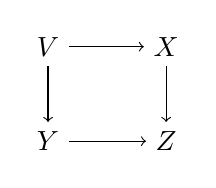
\begin{tikzpicture}
    \def\x{1.5}
    \def\y{-1.2}
    \node (A0_0) at (0*\x, 0*\y) {$V$};
    \node (A0_1) at (1*\x, 0*\y) {$X$};
    \node (A1_0) at (0*\x, 1*\y) {$Y$};
    \node (A1_1) at (1*\x, 1*\y) {$Z$};
    \path (A0_0) edge [->] node [auto] {$\scriptstyle{}$} (A0_1);
    \path (A1_0) edge [->] node [auto] {$\scriptstyle{}$} (A1_1);
    \path (A0_1) edge [->] node [auto] {$\scriptstyle{}$} (A1_1);
    \path (A0_0) edge [->] node [auto] {$\scriptstyle{}$} (A1_0);
  \end{tikzpicture}
  \]
  in una categoria $ℭ$ si dice \emph{cartesiano\/} se per ogni diagramma commutativo del tipo
  \[
  \begin{tikzpicture}
    \def\x{1.5}
    \def\y{-1.2}
    \node (A0_0) at (0*\x, 0*\y) {$V′$};
    \node (A1_1) at (1*\x, 1*\y) {$V$};
    \node (A1_2) at (2*\x, 1*\y) {$X$};
    \node (A2_1) at (1*\x, 2*\y) {$Y$};
    \node (A2_2) at (2*\x, 2*\y) {$Z$};
    \path (A0_0) edge [->,bend left=20] node [auto] {$\scriptstyle{}$} (A1_2);
    \path (A1_1) edge [->] node [auto] {$\scriptstyle{}$} (A1_2);
    \path (A0_0) edge [->,bend left=-20] node [auto] {$\scriptstyle{}$} (A2_1);
    \path (A1_1) edge [->] node [auto] {$\scriptstyle{}$} (A2_1);
    \path (A2_1) edge [->] node [auto] {$\scriptstyle{}$} (A2_2);
    \path (A1_2) edge [->] node [auto] {$\scriptstyle{}$} (A2_2);
  \end{tikzpicture}
  \]
  esiste unico un morfismo $V′ → V$ che commuta con il diagramma.
\end{definition}

In particolare, se $ℭ = \Sets$, dati $f\colon X → Z$ e $g\colon Y → Z$, possiamo definire il loro \emph{prodotto fibrato\/} come \[ X ×_Z Y ≔ \{(x,y) ∈ X × Y \mid f(x) = g(y)\}\text{;} \] è ben noto che il prodotto fibrato con le due proiezioni rende il diagramma cartesiano; inoltre ogni insieme che rende cartesiano il diagramma è isomorfo a $X ×_Z Y$, grazie alla proprietà universale.

Vogliamo trovare un'analoga proprietà universale per la cartesianità nel contesto delle $2$-categorie (o più in particolare, per i gruppoidi).

\begin{definition}
  Siano $f\colon X → Z$ e $g\colon Y → Z$ morfismi di gruppoidi; si definisce il \emph{prodotto fibrato\/}  
  \[\defcat{X ×_Z Y}{(x, y, φ)}{(x′, y′, φ′)}{
    \left\{\begin{array}{l} x ∈ \Obj(X), y ∈ \Obj(Y),\\ φ ∈ \Mor_Z(f(x),g(y))\end{array}\right.
  }{(α,β)}{
    \left\{\begin{array}{l}
    α ∈ \Mor_X(x, x′),\\
     β ∈ \Mor_Y(y, y′)\\
      \begin{tikzpicture}[baseline]
        \def\x{1.5}
        \def\y{-1.2}
        \node (A0_0) at (0*\x, -.5*\y) {$f(x)$};
        \node (A0_1) at (1*\x, -.5*\y) {$f(y)$};
        \node (A1_0) at (0*\x, .5*\y) {$g(x)$};
        \node (A1_1) at (1*\x, .5*\y) {$g(y)$};
        \node (A2_2) at (.5*\x, 0*\y) {$↻$};
        \path (A0_0) edge [->] node [auto] {$\scriptstyle{φ}$} (A0_1);
        \path (A1_0) edge [->] node [auto,swap] {$\scriptstyle{φ′}$} (A1_1);
        \path (A0_1) edge [->] node [auto] {$\scriptstyle{f(β)}$} (A1_1);
        \path (A0_0) edge [->] node [auto,swap] {$\scriptstyle{f(α)}$} (A1_0);
      \end{tikzpicture}
    \end{array}
  \right.
  }
\]
\end{definition}

\begin{lemma}
  Il prodotto fibrato ha una naturale struttura di gruppoide.
\end{lemma}

\begin{proof}
  L'identità dell'oggetto $(x, y, φ)$ è data da $(\id_x, \id_y)$; la composizione di \[ (x, y, φ) \xra{(α,β)} (x′, y′, φ′) \xra{(α′, β′)} (x″, y″, φ″) \] è $(α′∘α, β′∘β)$, ben definito in quanto
  \[
  \begin{tikzpicture}
    \def\x{2}
    \def\y{-1.6}
    \node (A0_0) at (0*\x, 0*\y) {$f(x)$};
    \node (A0_1) at (1*\x, 0*\y) {$g(y)$};
    \node (A1_0) at (0*\x, 1*\y) {$f(x′)$};
    \node (A1_1) at (1*\x, 1*\y) {$g(y′)$};
    \node (A2_0) at (0*\x, 2*\y) {$f(x″)$};
    \node (A2_1) at (1*\x, 2*\y) {$g(y″)$.};
    \path (A0_0) edge [->] node [auto] {$\scriptstyle{φ}$} (A0_1);
    \path (A0_1) edge [->,bend left=45] node [auto] {$\scriptstyle{g(β′∘β)}$} (A2_1);
    \path (A1_0) edge [->] node [auto] {$\scriptstyle{φ′}$} (A1_1);
    \path (A1_0) edge [->] node [auto] {$\scriptstyle{f(α′)}$} (A2_0);
    \path (A0_0) edge [->] node [auto] {$\scriptstyle{f(α)}$} (A1_0);
    \path (A0_0) edge [->,bend right=45] node [auto,swap] {$\scriptstyle{f(α′∘α)}$} (A2_0);
    \path (A0_1) edge [->] node [auto,swap] {$\scriptstyle{g(β)}$} (A1_1);
    \path (A2_0) edge [->] node [auto] {$\scriptstyle{φ″}$} (A2_1);
    \path (A1_1) edge [->] node [auto,swap] {$\scriptstyle{g(β′)}$} (A2_1);
  \end{tikzpicture}
  \]
  L'inverso di $(α, β)$ è $(α^{-1}, β^{-1})$.∎
\end{proof}

\begin{definition}
  Definiamo i funtori $p_1\colon X ×_Z Y → X$ e $p_2\colon X ×_Z Y → Y$ ponendo
  \begin{align*}
    p_1(x,y,z) &≔ x & p_1(α,β) &≔ α\text{,}\\
    p_2(x,y,z) &≔ y & p_2(α,β) &≔ β\text{.}
  \end{align*}
\end{definition}

Osserviamo che il diagramma 
  \[
  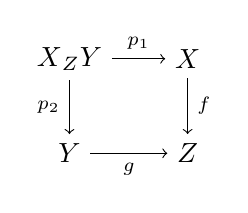
\begin{tikzpicture}
    \def\x{1.5}
    \def\y{-1.2}
    \node (A0_0) at (0*\x, 0*\y) {$X×_Z Y$};
    \node (A0_1) at (1*\x, 0*\y) {$X$};
    \node (A1_0) at (0*\x, 1*\y) {$Y$};
    \node (A1_1) at (1*\x, 1*\y) {$Z$};
    \path (A0_0) edge [->] node [auto] {$\scriptstyle{p_1}$} (A0_1);
    \path (A1_0) edge [->] node [auto,swap] {$\scriptstyle{g}$} (A1_1);
    \path (A0_1) edge [->] node [auto] {$\scriptstyle{f}$} (A1_1);
    \path (A0_0) edge [->] node [auto,swap] {$\scriptstyle{p_2}$} (A1_0);
  \end{tikzpicture}
  \]
in generale non commuta, dato che $f ∘ p_1(x,y,φ) = f(x)$ mentre $g∘p_2(x,y,φ) = g(y)$.

\begin{lemma}
  Esiste un'equivalenza naturale $ρ\colon p_1 ∘ f ⇒ p_2 ∘ g$ data da \[ ρ(x,y,φ) ≔ φ\colon f(x) → g(y)\text{.}\]
\end{lemma}

\begin{proof}
  Immediato dalla definizione di $X ×_Z Y$.∎
\end{proof}

L'ultima cosa da fare è adattare la proprietà universale di diagramma cartesiano alle $2$-categorie e dimostrare che il prodotto fibrato di gruppoidi la soddisfa.

\begin{theorem}\label{theorem:prodotto fibrato cartesiano}
  Sia
  \[
  \begin{tikzpicture}
    \def\x{1.5}
    \def\y{-1.2}
    \node (A0_0) at (0*\x, 0*\y) {$V$};
    \node (A0_1) at (1*\x, 0*\y) {$X$};
    \node (A1_0) at (0*\x, 1*\y) {$Y$};
    \node (A1_1) at (1*\x, 1*\y) {$Z$};
    \path (A0_0) edge [->] node [auto] {$\scriptstyle{q_1}$} (A0_1);
    \path (A0_0) edge [->] node [auto,swap] {$\scriptstyle{q_2}$} (A1_0);
    \path (A0_1) edge [->] node [auto] {$\scriptstyle{f}$} (A1_1);
    \path (A1_0) edge [->] node [auto,swap] {$\scriptstyle{g}$} (A1_1);
    \path (A1_0) -- (A0_1) 
      node [pos=0.5,sloped] {$\Longrightarrow$}
      node [pos=0.63,auto,sloped] {$\scriptstyle{η}$};
  \end{tikzpicture}
  \]
  un diagramma $2$-commutativo; allora esiste unica $h\colon V → X×_Y Z$ tale che
  \[
  \begin{tikzpicture}
    \def\x{1.5}
    \def\y{-1.2}
    \node (A0_0) at (0*\x, 0*\y) {$V$};
    \node (A1_1) at (1*\x, 1*\y) {$X ×_Z Y$};
    \node (A1_2) at (2*\x, 1*\y) {$X$};
    \node (A2_1) at (1*\x, 2*\y) {$Y$};
    \node (A2_2) at (2*\x, 2*\y) {$Z$};
    \path (A0_0) edge [->,bend left=40] node [auto] {$\scriptstyle{q_1}$} (A1_2);
    \path (A1_1) edge [->] node [auto] {$\scriptstyle{p_1}$} (A1_2);
    \path (A1_2) edge [->] node [auto] {$\scriptstyle{f}$} (A2_2);
    \path (A0_0) edge [->] node [auto,near start] {$\scriptstyle{h}$} (A1_1);
    \path (A1_1) edge [->] node [auto,swap] {$\scriptstyle{p_2}$} (A2_1);
    \path (A2_1) edge [->] node [auto,swap] {$\scriptstyle{g}$} (A2_2);
    \path (A0_0) edge [->,bend right=40] node [auto,swap] {$\scriptstyle{q_2}$} (A2_1);
    \path (A2_1) -- (A1_2) 
      node [pos=0.5,sloped] {$\Longrightarrow$}
      node [pos=0.63,auto,sloped] {$\scriptstyle{ρ}$};
    \path (0.1*\x,1.4*\y) -- (.7*\x,.7*\y) 
      node [pos=0.5,sloped] {$\Longrightarrow$}
      node [pos=0.63,auto,sloped] {$\scriptstyle{\id}$};
    \path (.7*\x,.7*\y) -- (1.4*\x,0.1*\y) 
      node [pos=0.5,sloped] {$\Longrightarrow$}
      node [pos=0.63,auto,sloped] {$\scriptstyle{\id}$};
  \end{tikzpicture}
  \]
  è $2$-commutativo; in particolare
  \begin{itemize}
    \item $q_1 = h ∘ p_1$,
    \item $q_2 = h ∘ p_2$,
    \item $ρ$ induce $η$.
  \end{itemize}  
\end{theorem}

\begin{proof}
  Il fatto che $η$ sia una trasformazione naturale che rende il primo diagramma $2$-commutativo si traduce in questo modo: \[ ∀ v ∈ \Obj(V), η(v)\colon f(q_1(v)) → g(q_2(v))\text{.} \] Dobbiamo definire $h(v)$: l'unica scelta plausibile è $h(v) ≔ (q_1(v), q_2(v), η(v))$, mentre per un morfismo $ψ\colon v_1 → v_2$, $h(ψ) ≔ (q_1(ψ), q_2(ψ))$. Rimangono da verificare che queste siano buone definizioni, in particolare che $h(ψ)$ sia un morfismo e che il diagramma
  \[
  \begin{tikzpicture}
    \def\x{2.5}
    \def\y{-1.6}
    \node (A0_0) at (0*\x, 0*\y) {$f(q_1(v_1))$};
    \node (A0_1) at (1*\x, 0*\y) {$g(q_2(v_1))$};
    \node (A1_0) at (0*\x, 1*\y) {$f(q_1(v_2))$};
    \node (A1_1) at (1*\x, 1*\y) {$g(q_2(v_2))$};
    \path (A0_0) edge [->] node [auto] {$\scriptstyle{η(v_1)}$} (A0_1);
    \path (A1_0) edge [->] node [auto,swap] {$\scriptstyle{η(v_2)}$} (A1_1);
    \path (A0_1) edge [->] node [auto] {$\scriptstyle{g(q_2(ψ))}$} (A1_1);
    \path (A0_0) edge [->] node [auto,swap] {$\scriptstyle{f(q_1(ψ))}$} (A1_0);
  \end{tikzpicture}
  \]
  commuta, cosa che è evidente dal fatto che $η$ è un'equivalenza naturale. L'ultima condizione, che $ρ$ induce $η$, si traduce semplicemente dicendo che l'ultima componente di $h(v)$ deve essere $η(v)$, come definito in precedenza.∎
\end{proof}

Abbiamo cambiato la proprietà universale, ma in un certo senso non molto: i $2$-morfismi in alto e a sinistra devono essere l'identità. In realtà quella esposta è una versione edulcorata della definizione di diagramma $2$-cartesiano.

\begin{definition}
  Un diagramma $2$-commutativo
  \[
  \begin{tikzpicture}
    \def\x{1.5}
    \def\y{-1.2}
    \node (A0_0) at (0*\x, 0*\y) {$V$};
    \node (A0_1) at (1*\x, 0*\y) {$X$};
    \node (A1_0) at (0*\x, 1*\y) {$Y$};
    \node (A1_1) at (1*\x, 1*\y) {$Z$};
    \path (A0_0) edge [->] node [auto] {$\scriptstyle{q_1}$} (A0_1);
    \path (A1_0) edge [->] node [auto,swap] {$\scriptstyle{g}$} (A1_1);
    \path (A0_1) edge [->] node [auto] {$\scriptstyle{f}$} (A1_1);
    \path (A0_0) edge [->] node [auto,swap] {$\scriptstyle{q_2}$} (A1_0);
    \path (A1_0) -- (A0_1) 
      node [pos=0.5,sloped] {$\Longrightarrow$}
      node [pos=0.63,auto,sloped] {$\scriptstyle{η}$};
  \end{tikzpicture}
  \]
  si dice \emph{$2$-cartesiano\/} se il funtore $h\colon V → X ×_Z Y$ definito nel Teorema~\ref{theorem:prodotto fibrato cartesiano} è un'equivalenza di gruppoidi.
\end{definition}

\begin{proposition}
  Un diagramma $2$-cartesiano ha la seguente proprietà universale: per ogni diagramma $2$-commutativo
  \[
  \begin{tikzpicture}
    \def\x{1.5}
    \def\y{-1.2}
    \node (A0_0) at (0*\x, 0*\y) {$V′$};
    \node (A0_1) at (1*\x, 0*\y) {$X$};
    \node (A1_0) at (0*\x, 1*\y) {$Y$};
    \node (A1_1) at (1*\x, 1*\y) {$Z$};
    \path (A0_0) edge [->] node [auto] {$\scriptstyle{q_1′}$} (A0_1);
    \path (A1_0) edge [->] node [auto,swap] {$\scriptstyle{g}$} (A1_1);
    \path (A0_1) edge [->] node [auto] {$\scriptstyle{f}$} (A1_1);
    \path (A0_0) edge [->] node [auto,swap] {$\scriptstyle{q_2′}$} (A1_0);
    \path (A1_0) -- (A0_1) 
      node [pos=0.5,sloped] {$\Longrightarrow$}
      node [pos=0.63,auto,sloped] {$\scriptstyle{η′}$};
  \end{tikzpicture}
  \]
  esiste un funtore $h′\colon V′ → V$ ed esistono dei $2$-morfismi $θ_1′\colon q_1 ∘ h′ ⇒ q_1′$ e $θ_2′\colon q_2 ∘ h′ ⇒ q_2′$ tale che
  \[
  \begin{tikzpicture}
    \def\x{1.5}
    \def\y{-1.2}
    \node (A0_0) at (0*\x, 0*\y) {$V′$};
    \node (A1_1) at (1*\x, 1*\y) {$V$};
    \node (A1_2) at (2*\x, 1*\y) {$X$};
    \node (A2_1) at (1*\x, 2*\y) {$Y$};
    \node (A2_2) at (2*\x, 2*\y) {$Z$};
    \path (A0_0) edge [->,bend left=40] node [auto] {$\scriptstyle{q_1′}$} (A1_2);
    \path (A1_1) edge [->] node [auto] {$\scriptstyle{q_1}$} (A1_2);
    \path (A1_2) edge [->] node [auto] {$\scriptstyle{f}$} (A2_2);
    \path (A0_0) edge [->] node [auto,near start] {$\scriptstyle{h′}$} (A1_1);
    \path (A1_1) edge [->] node [auto,swap] {$\scriptstyle{q_2}$} (A2_1);
    \path (A2_1) edge [->] node [auto,swap] {$\scriptstyle{g}$} (A2_2);
    \path (A0_0) edge [->,bend right=40] node [auto,swap] {$\scriptstyle{q_2′}$} (A2_1);
    \path (A2_1) -- (A1_2) 
      node [pos=0.5,sloped] {$\Longrightarrow$}
      node [pos=0.63,auto,sloped] {$\scriptstyle{ρ}$};
    \path (0.1*\x,1.4*\y) -- (.7*\x,.7*\y) 
      node [pos=0.5,sloped] {$\Longrightarrow$}
      node [pos=0.63,auto,sloped] {$\scriptstyle{θ_2′}$};
    \path (.7*\x,.7*\y) -- (1.4*\x,0.1*\y) 
      node [pos=0.5,sloped] {$\Longrightarrow$}
      node [pos=0.63,auto,sloped] {$\scriptstyle{θ_1′}$};
  \end{tikzpicture}
  \]
  induce $η′$. Inoltre $(h′, θ_1′, θ_2′)$ sono unici a meno di $2$-isomorfismo, cioè dati $(h″, θ_1″, θ_2″)$ con le stesse proprietà, esiste unico $δ\colon h′ ⇒ h″$ tale che il diagramma (visto prima da sopra e poi da sotto)
  \begin{align*}
  &\begin{tikzpicture}
    \def\x{1.2}
    \def\y{3}
    \node (A0_0) at (0*\x, 1*\y) {$V′$};
    \node (A0_1) at (0*\x, 0*\y) {$X$};
    \path (A0_0) edge [->,bend left=70] node [auto] {$\scriptstyle{q_1 ∘ h′}$} (A0_1);
    \path (A0_0) edge [->] node [auto,near end] {$\scriptstyle{q_1′}$} (A0_1);
    \path (A0_0) edge [->,bend right=70] node [auto,swap] {$\scriptstyle{q_1∘ h″}$} (A0_1);
    \path (-1*\x, 0.5*\y) -- (0*\x, 0.5*\y) 
      node [pos=0.5,sloped] {$\Longrightarrow$}
      node [pos=0.5,auto,sloped] {$\scriptstyle{θ_1′}$};
    \path (1*\x, 0.5*\y) -- (0*\x, 0.5*\y) 
      node [pos=0.5,allow upside down,sloped] {$\Longrightarrow$}
      node [pos=0.5,auto,swap,sloped] {$\scriptstyle{θ_1″}$};
  \end{tikzpicture}
  &&\begin{tikzpicture}
    \def\x{1.2}
    \def\y{3}
    \node (A0_0) at (0*\x, 1*\y) {$V′$};
    \node (A0_1) at (0*\x, 0*\y) {$X$};
    \path (A0_0) edge [->,bend left=70] node [auto] {$\scriptstyle{q_1 ∘ h″}$} (A0_1);
    \path (A0_0) edge [->,bend right=70] node [auto,swap] {$\scriptstyle{q_1∘ h′}$} (A0_1);
    \path (0.5*\x, 0.5*\y) -- (-0.5*\x, 0.5*\y) 
      node [pos=0.5,allow upside down,sloped] {$\Longrightarrow$}
      node [pos=0.5,auto,swap,sloped] {$\scriptstyle{q_1(δ)}$};
  \end{tikzpicture}
  \end{align*}
  sia $2$-commutativo, e allo stesso modo per $θ_2′$ e $θ_2″$.
\end{proposition}

È possibile usare la semplificazione vista all'inizio in quanto si dimostra che tra questi dati ne esiste sempre uno con $θ_1′ = \id$ e $θ_2′ = \id$.

\begin{exercise}
  Se $X$, $Y$, $Z$ sono insiemi e $X′$, $Y′$, $Z′$ sono gli stessi insiemi visti come gruppoidi, allora $X′ ×_{Z′} Y′$ è l'insieme $X ×_Z Y$ visto come gruppoide
\end{exercise}

\begin{proof}[Soluzione.]
  Sia $(x, y, φ) ∈ X′ ×_{Z′} Y′$, cioè $x ∈ X$, $y ∈ Y$ e $φ\colon f(x) → g(y)$; allora $f(x) = g(y)$ e $φ = \id$, dato che $Z$ è un insieme; mentre un morfismo da $(x, y, \id_{f(x)}$ a $(x′, y′, \id_{f(x′)})$ può essere solo $(\id_x, \id_{y})$ se $x = x′$ e $y = y′$.∎
\end{proof}

\begin{exercise}
  Il prodotto fibrato è stabile, modulo equivalenza, sostituendo $X$, $Y$, $Z$ con gruppoidi equivalenti. Per esempio, se $a\colon X′ → X$ è un'equivalenza naturale, allora $a$ induce un'equivalenza $X′×_Z Y → X×_Z Y$; lo stesso per $b\colon Y′ → Y$ e $c\colon Z → Z′$.
\end{exercise}

%\begin{proof}[Soluzione]
%  Sia $σ\colon X′ → X$ un'equivalenza naturale e consideriamo il diagramma
%  \[
%  \begin{tikzpicture}
%    \def\x{1.5}
%    \def\y{-1.2}
%    \node (A0_0) at (0*\x, 0*\y) {$X′ ×_Z Y$};
%    \node (A0_1) at (1*\x, 0*\y) {$X′$};
%    \node (A1_0) at (0*\x, 1*\y) {$X ×_Z Y$};
%    \node (A1_1) at (1*\x, 1*\y) {$X$};
%    \node (A2_0) at (0*\x, 2*\y) {$Y$};
%    \node (A2_1) at (1*\x, 2*\y) {$Z$.};
%    \path (A0_0) edge [->] node [auto] {$\scriptstyle{q_1′}$} (A0_1);
%    \path (A2_0) edge [->] node [auto,swap] {$\scriptstyle{g}$} (A2_1);
%    \path (A1_0) edge [->] node [auto] {$\scriptstyle{q_1}$} (A1_1);
%    \path (A1_0) edge [->] node [auto,swap] {$\scriptstyle{q_2}$} (A2_0);
%    \path (A1_1) edge [->] node [auto] {$\scriptstyle{f}$} (A2_1);
%    \path (A0_0) edge [->,bend right=60] node [auto,swap] {$\scriptstyle{q_2′}$} (A2_0);
%    \path (A0_1) edge [->] node [auto] {$\scriptstyle{σ}$} (A1_1);
%  \end{tikzpicture}
%  \]
%  Definiamo un'equivalenza $τ\colon X′×_Z Y → X×_Z Y$ ponendo
%  \begin{align*}
%    τ(x′,y,φ) &≔ (σ(x′), y, φ)\text{,} & τ(α′, β) &≔ (σ(α′), β)\text{.}
%  \end{align*}
%  Si procede allo stesso modo per $Y$ e $Z$.∎
%\end{proof}

\begin{proposition}
  Sia $G$ un gruppoide che agisce su un insieme $X$. Denotiamo $X′$ il gruppoide associato a $X$; definiamo $π\colon X′ → [X/G]$ ponendo
  \begin{align*}
    π(x) &≔ x\text{,} & π(\id_x) &≔ \id_x\text{,}
  \end{align*}
  $p_2\colon G × X′ → X′$ con $p_2(g, x) ≔ x$ e $a\colon G×X′ → X′$ con $a(g, x) ≔ g⋅x$. Il diagramma 
  \[
  \begin{tikzpicture}
    \def\x{1.5}
    \def\y{-1.2}
    \node (A0_0) at (0*\x, 0*\y) {$G×X′$};
    \node (A0_1) at (1*\x, 0*\y) {$X′$};
    \node (A1_0) at (0*\x, 1*\y) {$X′$};
    \node (A1_1) at (1*\x, 1*\y) {$[X/G]$};
    \path (A0_0) edge [->] node [auto] {$\scriptstyle{a}$} (A0_1);
    \path (A0_0) edge [->] node [auto,swap] {$\scriptstyle{p_2}$} (A1_0);
    \path (A0_1) edge [->] node [auto] {$\scriptstyle{π}$} (A1_1);
    \path (A1_0) edge [->] node [auto,swap] {$\scriptstyle{π}$} (A1_1);
    \path (A1_0) -- (A0_1) 
      node [pos=0.5,sloped] {$\Longrightarrow$}
      node [pos=0.63,auto,sloped] {$\scriptstyle{η}$};
  \end{tikzpicture}
  \]
  è naturalmente $2$-commutativo tramite un $2$-morfismo $η$, che inoltre rende il diagramma cartesiano.
\end{proposition}

\begin{proof}
  Sia $(g, x) ∈ \Obj(G × X′)$; allora $(π∘p_2)(g,x) = x$, mentre $(π∘p_1)(g,x) = g⋅x$; l'unico modo per definire $η$ è ponendo $η(g,x) ≔ g ∈ \Mor_{[X/G]}(x, g⋅x)$.
  
  Sia ora $Y$ il prodotto fibrato $X′ ×_{[X/G]} X′$; i suoi oggetti sono triple $(x_1, x_2, g)$ con $x_1, x_2 ∈ X$ e $g ∈ G$ tale che $g⋅x_1 = x_2$. I morfismi tra $(x_1, x_2, g)$ e $(x_1′, x_2′, g′)$ sono coppie di morfismi $x_1 → x_1′$ e $x_2 → x_2′$, quindi necessariamente, dato che $X$ è un insieme, non ci sono morfismi se $x_1 ≠ x_1′$ o $x_2 ≠ x_2′$; inoltre, perché $(\id_{x_1}, \id_{x_2})$ sia davvero un morfismo, il diagramma
  \[
  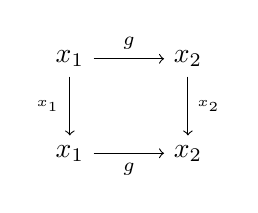
\begin{tikzpicture}
    \def\x{1.5}
    \def\y{-1.2}
    \node (A0_0) at (0*\x, 0*\y) {$x_1$};
    \node (A0_1) at (1*\x, 0*\y) {$x_2$};
    \node (A1_0) at (0*\x, 1*\y) {$x_1$};
    \node (A1_1) at (1*\x, 1*\y) {$x_2$};
    \path (A0_0) edge [->] node [auto] {$\scriptstyle{g}$} (A0_1);
    \path (A0_0) edge [->] node [auto,swap] {$\scriptstyle{\id_{x_1}}$} (A1_0);
    \path (A0_1) edge [->] node [auto] {$\scriptstyle{\id_{x_2}}$} (A1_1);
    \path (A1_0) edge [->] node [auto,swap] {$\scriptstyle{g}$} (A1_1);
  \end{tikzpicture}
  \]
  deve commutare. In definitiva, gli unici morfismi sono le identità se le due triple sono uguali, cioè $Y$ è un insieme. L'applicazione $G×X′ → Y$, indotta dal fatto che $Y$ è un prodotto fibrato, è data da $(g,x) ↦ (x, g⋅x, g)$, come applicazione tra insiemi, che è chiaramente biunivoca (l'inversa dimentica il secondo elemento della tripla).∎
\end{proof}

Ritornando agli insiemi, consideriamo l'azione di un gruppo $G$ su un insieme $X$. Possiamo costruire un insieme quoziente $X/G$ e un diagramma commutativo
  \[
  \begin{tikzpicture}
    \def\x{1.5}
    \def\y{-1.2}
    \node (A0_0) at (0*\x, 0*\y) {$G×X$};
    \node (A0_1) at (1*\x, 0*\y) {$X$};
    \node (A1_0) at (0*\x, 1*\y) {$X$};
    \node (A1_1) at (1*\x, 1*\y) {$X/G$};
    \path (A0_0) edge [->] node [auto] {$\scriptstyle{a}$} (A0_1);
    \path (A0_0) edge [->] node [auto,swap] {$\scriptstyle{p_2}$} (A1_0);
    \path (A0_1) edge [->] node [auto] {$\scriptstyle{π}$} (A1_1);
    \path (A1_0) edge [->] node [auto,swap] {$\scriptstyle{π}$} (A1_1);
  \end{tikzpicture}
  \]
dove $a$ è l'azione e $p_2$ la proiezione.

\begin{exercise}
  Il diagramma è cartesiano se e solo se l'azione di $G$ è libera (cioè se ogni stabilizzatore è banale).\TODO{}
\end{exercise}

%\begin{proof}[Soluzione.]
%  Sia \[ Y ≔ X ×_{X/G} X = \{(x_1, x_2) \mid ∃ g ∈ G\colon g x_1 = x_2 \}\text{;} \] se $O_1, …$ sono le orbite di $G$ in $X$, $Y = \bigsqcup O_i × O_i$. Consideriamo la mappa $f\colon G×X → X×X$ con $f(g,x) ≔ (g⋅x, x)$. Se l'azione è libera, $f$ è iniettiva, e la sua immagine è $Y$, quindi il diagramma è cartesiano. Viceversa, se il diagramma è cartesiano, esiste un isomorfismo $f\colon G×X → Y$. Se per assurdo l'azione non fosse libera, esisterebbe $(g,x) ∈ G×X$ tale che $g⋅x = x$ e $g ≠ e$. In particolare, $p_2(e,x) = x = p_2(g,x)$ e $a(e,x) = x = a(g,x)$. Ma allora $q_i(f(e,x)) = q_i(f(g,x))$ per $i ∈\{1,2\}$, dove $q_1, q_2\colon Y → X$ sono le due proiezioni; di conseguenza, $f(e,x) = f(g,x)$ assurdo.∥∎
%\end{proof}

\begin{remark}
  Sia $x ∈ \Obj([X/G])$; allora $\Aut(x) = \Stab_G(x)$. Quindi considerando i gruppoidi, tutte le azioni di gruppo si comportano come un'azione libera.
\end{remark}

\begin{definition}
  Sia $G$ un gruppoide; il \emph{gruppoide d'inerzia\/} associato a $G$ è
  \[\defcat{\I(G)}{(x, φ)}{(y, ψ)}{x ∈ \Obj(G), φ ∈ \Aut(x)}{σ\colon x → y}{
  \begin{tikzpicture}[baseline]
    \def\x{1}
    \def\y{-0.8}
    \node (A0_0) at (0*\x, -.5*\y) {$x$};
    \node (A0_1) at (1*\x, -.5*\y) {$x$};
    \node (A1_0) at (0*\x, .5*\y) {$y$};
    \node (A1_1) at (1*\x, .5*\y) {$y$};
    \node (A2_2) at (.5*\x, 0*\y) {$↻$};
    \path (A0_0) edge [->] node [auto] {$\scriptstyle{φ}$} (A0_1);
    \path (A0_0) edge [->] node [auto,swap] {$\scriptstyle{σ}$} (A1_0);
    \path (A0_1) edge [->] node [auto] {$\scriptstyle{σ}$} (A1_1);
    \path (A1_0) edge [->] node [auto,swap] {$\scriptstyle{ψ}$} (A1_1);
  \end{tikzpicture}}\]
  inoltre si definisce una proiezione $π\colon \I(G) → G$ ponendo $π(x, φ) ≔ x$ e $π(σ) ≔ σ$.
\end{definition}

\begin{exercise}
  Esiste un naturale $2$-morfismo $η$ che rende il diagramma
  \[
  \begin{tikzpicture}
    \def\x{1.5}
    \def\y{-1.2}
    \node (A0_0) at (0*\x, 0*\y) {$\I(G)$};
    \node (A0_1) at (1*\x, 0*\y) {$G$};
    \node (A1_0) at (0*\x, 1*\y) {$G$};
    \node (A1_1) at (1*\x, 1*\y) {$G×G$};
    \path (A0_0) edge [->] node [auto] {$\scriptstyle{π}$} (A0_1);
    \path (A0_0) edge [->] node [auto,swap] {$\scriptstyle{π}$} (A1_0);
    \path (A0_1) edge [->] node [auto] {$\scriptstyle{Δ_G}$} (A1_1);
    \path (A1_0) edge [->] node [auto,swap] {$\scriptstyle{Δ_G}$} (A1_1);
    \path (A1_0) -- (A0_1) 
      node [pos=0.5,sloped] {$\Longrightarrow$}
      node [pos=0.63,auto,sloped] {$\scriptstyle{η}$};
  \end{tikzpicture}
  \]
  $2$-cartesiano.  
\end{exercise}

\begin{proof}[Solution.]
  We have to define $η_{(x,φ)}\colon (x,x) → (x,x)$, that is, $η_{(x,φ)} = (α_{(x,φ)}, β_{(x,φ)})$. Moreover, both $α$ and $β$ have to commute with any morphism $σ\colon x → y$. The natural answer is to set $α_{(x,φ)} = φ = β_{(x, φ)}$, since $φ$ commutes with $σ$ by definition of $\I(G)$.∎
\end{proof}

\section{Schemes as functors}\lecture[2 hours]{15}{01}{2009}
As we said, after defining groupoids and seeing some of their properties, we need to reshape the definition of scheme in order to make evident the fact that their morphisms form a set. The key to do this is Yoneda lemma.

\begin{definition}
  If $ℭ$ is any category, there is a natural functor \[ \ho\colon ℭ → \Fun(ℭ^{\opp}, \Sets) \] associating to an object $X$ the functor $\ho_X$ defined by \[ \ho_X(Y) ≔ \Mor_ℭ(Y, X)\text{,} \qquad \ho_X(f\colon Y → Z)\colon \Mor_ℭ(Z, X) \xra{(\pha∘f)} \Mor_ℭ(Y, X)\text{.} \]
\end{definition}

\begin{lemma}[Yoneda]
  The natural map $\Mor(\ho_X, F) → F(X)$ associating $α(\id_X)$ to $α\colon \ho_X ⇒ F$ is a bijection for every $F\colon ℭ^\opp → \Sets$.
\end{lemma}

\begin{corollary}
  The functor $\ho$ is fully faithful.
\end{corollary}

\begin{proof}
  By Yoneda lemma, $\Mor(\ho_X, \ho_Y)$ is bijective to $\ho_Y(X) ≔ \Mor(X, Y)$.
\end{proof}

\begin{definition}
  A functor $F\colon ℭ^{\opp} → \Sets$ is called \emph{representable\/} if there exist $X ∈ \Obj(ℭ)$ and $α ∈ F(X)$ (that is, $α\colon \ho_X ⇒ F$) such that $α$ is a natural equivalence. In such a situation, we say that $X$ (or better, the couple $(X, α)$) \emph{represents\/} $F$.
\end{definition}

We can view the property that fibered product is defined up to canonical isomorphism in another way thanks to representability.

\begin{lemma}
  If both $(X, α)$ and $(X′, α′)$ represent $F$, then there is an unique isomorphism $f\colon X → X′$ such that the diagram
  \[
  \begin{tikzpicture}
    \def\x{0.8}
    \def\y{-1.2}
    \node (A0_0) at (150:\x) {$\ho_X$};
    \node (A0_2) at (30:\x) {$\ho_{X′}$};
    \node (A1_1) at (270:\x) {$F$};
    \path (A0_0) edge [->] node [auto,swap] {$\scriptstyle{α}$} (A1_1);
    \path (A0_2) edge [->] node [auto] {$\scriptstyle{α′}$} (A1_1);
    \path (A0_0) edge [->] node [auto] {$\scriptstyle{f}$} (A0_2);
  \end{tikzpicture}
  \]
  commutes.
\end{lemma}

In particular, there could be many isomorphisms, but only one commutes with $α$ and $α′$.

\begin{definition}
  Let $ℭ$ be a category; we say that \emph{fiber products exist\/} in $ℭ$ if we can complete every diagram
  \[
  \begin{tikzpicture}
    \def\x{1.5}
    \def\y{-1.2}
    \node (A0_1) at (1*\x, 0*\y) {$X$};
    \node (A1_0) at (0*\x, 1*\y) {$Y$};
    \node (A1_1) at (1*\x, 1*\y) {$Z$};
    \path (A1_0) edge [->] node [auto] {$\scriptstyle{}$} (A1_1);
    \path (A0_1) edge [->] node [auto] {$\scriptstyle{}$} (A1_1);
  \end{tikzpicture}
  \]  
  to a cartesian diagram
  \[
  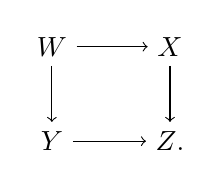
\begin{tikzpicture}
    \def\x{1.5}
    \def\y{-1.2}
    \node (A0_0) at (0*\x, 0*\y) {$W$};
    \node (A0_1) at (1*\x, 0*\y) {$X$};
    \node (A1_0) at (0*\x, 1*\y) {$Y$};
    \node (A1_1) at (1*\x, 1*\y) {$Z$.};
    \node (B1_1) at (.5*\x, .5*\y) {$\square$};
    \path (A0_0) edge [->] node [auto] {$\scriptstyle{}$} (A0_1);
    \path (A1_0) edge [->] node [auto] {$\scriptstyle{}$} (A1_1);
    \path (A0_1) edge [->] node [auto] {$\scriptstyle{}$} (A1_1);
    \path (A0_0) edge [->] node [auto] {$\scriptstyle{}$} (A1_0);
  \end{tikzpicture}
  \]
\end{definition}  

\begin{lemma}
  For any category $ℭ$, the category $\Fun(ℭ^{\opp}, \Sets)$ has fiber products.
\end{lemma}

\begin{proof}
  Given such a diagram, let $W(A) ≔ X(A) ×_{Z(A)} Y(A)$; for a morphism $f\colon A → B$, we have projections $W(B) → X(B)$ and $W(B) → Y(B)$ and also the maps $X(f)\colon X(B) → X(A)$ and $Y(f)\colon Y(B) → Y(A)$; since $W(B)$ is a fiber product, we have an induced map $W(f)\colon W(B) → W(A)$. It is an easy check that $W$ is a functor and that there are natural morphisms $W → X$ and $W → Y$ such that $W$ with these morphisms complete a cartesian diagram.∎
\end{proof}

\begin{exercise}
  A category $ℭ$ has fiber product if and only if for every $f\colon X → Z$ and $g\colon Y → Z$, the functor $\ho_X ×_{\ho_Z} \ho_Y$ is representable.
\end{exercise}

\begin{proof}[Solution.]
  Let $F ≔ \ho_X ×_{\ho_Z} \ho_Y$; if $F$ is representable, $F$ is naturally equivalent to $\ho_W$ for some $W ∈ \Obj(ℭ)$. Via this equivalence, we have that $\id_W ∈ \ho_W(W)$ corresponds to some element $α ∈ F(W)$; but $F(W)$ has two projections $p_1$ and $p_2$ to $\ho_X$ and $\ho_Y$, so we define $q_1 ≔ p_1(W)(α)$ and $q_2 ≔ p_2(W)(α)$. These morphisms make the diagram commute, since $\ho(f) ∘ p_1 = \ho(g) ∘ p_2$. Moreover the diagram is cartesian since from $(V, s_1\colon V → X, s_2\colon V → Y)$ we get morphisms $\ho(s_1)\colon \ho_V ⇒ \ho_X$ and $\ho(s_2)\colon \ho_V ⇒ \ho_X$ and by cartesianity a morphism $τ\colon \ho_V ⇒ \ho_W$; from this, the desired morphism $τ(V)(\id_V)$.
  
  Viceversa, if $X ×_Z Y$ exists, it represents of $\ho_X ×_{\ho_Y} \ho_Z$.∎
\end{proof}

In some sense, we proved that if we enlarge enough the category (for example considering the larger category of contravariant functors to $\Sets$) we can always assume that we work in a category with fiber products.

Thanks to Yoneda lemma, we know that we can think a scheme as a contravariant functor from schemes to sets. This seems a bit circular, so we try to replace this with some precedent object. In particular, we assume to know affine schemes and we consider for a generic scheme $X$ the restriction of $\ho_X$ to affine schemes: \[ \ho_X\colon \AffineSchemes^{\opp} → \Sets\text{.} \]

\begin{remark}
  As in Yoneda lemma, we get functors \[ \Schemes → \Fun(\AffineSchemes^{\opp} → \Sets)\text{,}\] but this could be no longer an equivalence.
\end{remark}

\begin{theorem}\label{theorem:affine schemes are enough}
  \mbox{}
  \begin{enumerate}
    \item This functor is a fully faithful;
    \item we can characterize its essential image, that is, we can describe which functors are isomorphic to $\ho_X$ for some scheme $X$, without using the definition of schemes.
  \end{enumerate}
\end{theorem}

\begin{corollary}
  Schemes forms a full subcategory of $\Fun(\AffineSchemes^\opp, \Sets)$.
\end{corollary}

So we can define scheme in a complete different way from the usual one, assuming only the knowledge of affine schemes (or equivalently finitely generated $K$-algebras). A way to understand this, is to think that a functor $\AffineSchemes^\opp → \Sets$ encodes all possible charts from some affine schemes to our yet to be defined scheme, instead of just selecting some of them as we do in the usual way.

\begin{proof}[Proof of Theorem~\ref{theorem:affine schemes are enough}, part 1]
  Let $X$ and $Y$ be schemes so that $\ho_X, \ho_Y\colon \AffineSchemes^{\opp} → \Sets$. We have to prove that $\Mor(X, Y) → \Mor(\ho_X, \ho_Y)$ is a bijection; to do so we provide an inverse.
  
  Assume $X$ is separated; in particular, for every $U, V ⊆ X$ open affine, also $U∩V$ is open and affine; choose an open affine cover $\{U_i\mid i ∈ I\}$ of $X$ via inclusions $α_i\colon U_i → X$. Let $f\colon \ho_X → \ho_Y$; then $f(α_i) ∈ \ho_Y(U_i)$, that is $f(α_i)\colon U_i → Y$. As usual define $U_{i,j} ≔ U_i ∩ U_j$, with injections $s_{i,j}\colon U_{i,j} → U_i$ and $t_{i,j}\colon U_{i,j} → U_j$. Then 
  \[
  \begin{tikzpicture}
    \def\x{1.5}
    \def\y{-1.2}
    \node (A0_1) at (1*\x, 0*\y) {$U_i$};
    \node (A1_0) at (0*\x, 1*\y) {$U_{i,j}$};
    \node (A1_2) at (2*\x, 1*\y) {$X$};
    \node (A2_1) at (1*\x, 2*\y) {$U_j$};
    \path (A1_0) edge [->] node [auto] {$\scriptstyle{α_{i,j}}$} (A1_2);
    \path (A1_0) edge [->] node [auto,swap] {$\scriptstyle{t_{i,j}}$} (A2_1);
    \path (A0_1) edge [->] node [auto] {$\scriptstyle{α_i}$} (A1_2);
    \path (A2_1) edge [->] node [auto,swap] {$\scriptstyle{α_j}$} (A1_2);
    \path (A1_0) edge [->] node [auto] {$\scriptstyle{s_{i,j}}$} (A0_1);
  \end{tikzpicture}
  \]
  commutes and we get maps $s_{i,j}^⋆\colon \ho_X(U_i) → \ho_X(U_{i,j})$ and $t_{i,j}^⋆\colon \ho_X(U_j) → \ho_X(U_{i,j})$ that, applying $f$, we have \[ {f(α_i)}_{|U_{i,j}} = f(α_i) ∘ s_{i,j}^⋆ = f(α_{i,j}) = f_(α_j) ∘ t_{i,j}^⋆ = {f(α_j)}_{|U_{i,j}}\text{.}\] Therefore we can define $g\colon X → Y$ in such a way that $g_{|U_i} = f(α_i)$ and $g$ is a uniquely determined morphism of schemes. It is now easy to check that this is really the inverse.
  
  In the nonseparated case, the argument is the same but we have to cover again the intersections $U_{i,j}$ by affine open sets and the proof is just notationally more complicated.∎
\end{proof}

Then taking either all schemes or only affine schemes, we get two equivalent categories $\Fun(\Schemes^{\opp}, \Sets)$ and $\Fun(\AffineSchemes^{\opp}, \Sets)$. To prove the second part of Theorem~\ref{theorem:affine schemes are enough}, we need a criterion which tell us when a functor is in the essential image of $\ho$. The key concept is the next proposition, which will be proved later.

\begin{proposition}
  Let $X$ be a scheme; then the functor $\ho_X$ is a sheaf in the Zariski topology on $\AffineSchemes$ in the following sense: if $S$ is an affine schemes and $\{U_i \mid i ∈ I\}$ is an affine open cover of $S$ (in particular, $U_{i,j}$ are also open affine), then the sequence
  \[
  \begin{tikzpicture}
    \def\x{2.8}
    \def\y{-1.2}
    \node (A0_0) at (0*\x, 0*\y) {$\pha$};
    \node (A0_1) at (1*\x, 0*\y) {$\ho_X(S)$};
    \node (A0_2) at (2*\x, 0*\y) {$∏ \ho_X(U_i)$};
    \node (A0_3) at (3*\x, 0*\y) {$∏ \ho_X(U_{i,j})$};
    \path (A0_0) edge [->] node [auto] {$\scriptstyle{}$} (A0_1);
    \path (A0_2) edge [->,bend left=10] node [auto] {$\scriptstyle{\ho_X(s_{i,j})}$} (A0_3);
    \path (A0_2) edge [->,bend right=10] node [auto,swap] {$\scriptstyle{\ho_X(t_{i,j})}$} (A0_3);
    \path (A0_1) edge [->] node [auto] {$\scriptstyle{\ho_X(α_i)}$} (A0_2);
  \end{tikzpicture}
  \]
  is exact. This means that $\ho_X(α_i)$ is injective and its image is the locus where the two other maps coincide. In other words, given for every $i∈I$ morphisms $f_i ∈ \ho_X(U_i)$, then exists $f ∈ \ho_X(S)$ such that $f_{|U_i} = f_i$ (or $\ho_X(α_i)(f) = f_i$) if and only if ${f_i}_{|U_{i,j}} = {f_j}_{|U_{i,j}}$ (or $\ho_X(s_{i,j})(f_i) = \ho_X(t_{i,j})(f_j)$); if so, then $f$ is unique.
\end{proposition}

Another important and more difficult theorem is that $\ho_X$ is a sheaf also in the étale topology.

So far we have shown that the category of schemes is equivant to a full subcategory of the category of sheaves of sets on $\AffineSchemes$ for the Zariski (and we said it is true also for étale) topology. In particular we found what we were searching: now it is evident that morphisms of schemes forms a set, since the sheaves are of sets. How do we define sheaves of groupoids? The notion of presheaf of sets is just the one of contravariant functor to $\Sets$; then a presheaf of groupoids is just a contravariant functor to $\Groupoids$, adapted to the fact that groupoids form a $2$-category. After that we have to add glueing conditions to make a sheaf, but we will see these later.

One could ask if this is the best path to define stacks. Couldn't there be a definition that starts from a topological spaces like the objects we are acquainted to? Sure it is possible to associate a topological space to every stack; in particular orbifolds (that are, complex or symplectic manifolds that are equivalent to Deligne-Mumford stacks) are defined starting from a topological space. Indeed the definition of orbifold is much easier but it has an important problem.

\begin{problem}
  With the orbifold approach, the objects are very easy to define, the morphisms are messy and the $2$-morphisms are yet not defined.
\end{problem}

So let's go back to our path to the definition of presheaves of groupoids.

\begin{definition}
  Let $ℭ$ be a category; a \emph{pseudofunctor\/} from $ℭ$ to $\Groupoids$ is denoted as $F\colon ℭ → \Groupoids$ and is the data of:
  \begin{itemize}
    \item for every $X ∈ \Obj(ℭ)$, a groupoid $F(X)$;
    \item for every $f\colon X → Y$, a functor $F(f)\colon F(Y) → F(X)$.
    \item for every sequence $X \xra{f} Y \xra{g} Z$, a $2$-commutative diagram
  \[
  \begin{tikzpicture}
    \def\x{1.2}
    \def\y{-1.2}
    \node (A0_0) at (150:\x) {$F(X)$};
    \node (A0_2) at (30:\x) {$F(Z)$};
    \node (A1_1) at (270:\x) {$F(Y)$};
    \path (A1_1) edge [->] node [auto] {$\scriptstyle{F(f)}$} (A0_0);
    \path (A0_2) edge [->] node [auto] {$\scriptstyle{F(g)}$} (A1_1);
    \path (A0_2) edge [->] node [auto,swap] {$\scriptstyle{F(g∘f)}$} (A0_0);
    \path (273:\x) -- (80:0.9*\x) 
      node [pos=0.5,sloped] {$\Longrightarrow$}
      node [pos=0.63,auto,sloped] {$\scriptstyle{α_{f,g}}$};
  \end{tikzpicture}
  \]
  \end{itemize}
  The data is subject to these conditions:
  \begin{itemize}
    \item $F(\id_X) = \id_{F(X)}$;
    \item when either $f$ or $g$ is the identity, then $α_{f,g}$ is the identity;
    \item for every sequence $X \xra{f} Y \xra{g} Z \xra{h} W$, a $2$-commutative tetrahedron (seen from above and from the bottom)
  \begin{align*}
  &\begin{tikzpicture}[baseline]
    \def\x{2}
    \def\y{-1.2}
    \node (A0_0) at (150:\x) {$F(X)$};
    \node (A0_2) at (30:\x) {$F(Z)$};
    \node (A1_1) at (0:0) {$F(W)$};
    \node (A2_1) at (270:\x) {$F(Y)$};
    \path (A1_1) edge [->] node [auto,very near start] {$\scriptstyle{F(h∘g∘f)}$} (A0_0);
    \path (A1_1) edge [->] node [auto,near end] {$\scriptstyle{F(h)}$} (A0_2);
    \path (A0_2) edge [->,bend right=45] node [auto,swap] {$\scriptstyle{F(g∘f)}$} (A0_0);
    \path (A0_2) edge [->,bend left=45] node [auto] {$\scriptstyle{F(g)}$} (A2_1);
    \path (A1_1) edge [->] node [auto,near end] {$\scriptstyle{F(h∘g)}$} (A2_1);
    \path (A2_1) edge [->,bend left=45] node [auto] {$\scriptstyle{F(f)}$} (A0_0);
    \path (A0_2) -- (A0_0) 
      node [pos=0.6,allow upside down,sloped] {$\Longrightarrow$}
      node [pos=0.6,auto,sloped] {$\scriptstyle{α_{g∘f,h}}$};
    \path (A2_1) -- (A0_0) 
      node [pos=0.35,allow upside down,sloped] {$\Longrightarrow$}
      node [pos=0.2,auto,sloped] {$\scriptstyle{α_{f,h∘g}}$};
    \path (A0_2) -- (A2_1) 
      node [pos=0.4,allow upside down,sloped] {$\Longrightarrow$}
      node [pos=0.5,auto,sloped] {$\scriptstyle{α_{h,g}}$};
  \end{tikzpicture}
  &&\begin{tikzpicture}[baseline]
    \def\x{2}
    \def\y{-1.2}
    \node (A0_0) at (150:\x) {$F(Z)$};
    \node (A0_2) at (30:\x) {$F(X)$};
    \node (A2_1) at (270:\x) {$F(Y)$};
    \path (A0_0) edge [->,bend left=45] node [auto] {$\scriptstyle{F(g∘f)}$} (A0_2);
    \path (A2_1) edge [->,bend right=45] node [auto,swap] {$\scriptstyle{F(f)}$} (A0_2);
    \path (A0_0) edge [->,bend right=45] node [auto,swap] {$\scriptstyle{F(g)}$} (A2_1);
    \path (273:\x) -- (80:0.9*\x) 
      node [pos=0.5,sloped] {$\Longrightarrow$}
      node [pos=0.53,auto,sloped] {$\scriptstyle{α_{f,g}}$};
  \end{tikzpicture}
  \end{align*}
      and we ask that the two $2$-commutative diagrams commutes.
  \end{itemize}
\end{definition}

The definition is the natural extension of the one of functors, once changed equalities of functors to $2$-isomorphisms. Actually, the first two condition do not follow this convention, but one sees that keeping this equalities does not rule out an important part of functors.

We encounter this approach every time we mess with groupoids and $2$-category: we change equality to $2$-isomorphisms, and request compatibility on the superior level. If for functors the data are something for every object and every arrow, subject to a condition on a sequence of two arrows, for pseudofunctors the data are something for every object, every arrow and every sequence of two arrows, subject to a condition for every sequence of three arrows.

\begin{example}
  Consider the mapping $V\colon \Manifolds → \Groupoids$ where:
  \begin{itemize}
    \item $V(M)$ is the groupoids with objects rank $r$ vector bundles on $M$ and morphisms are isomorphisms of vector bundles;
    \item for every $f\colon M → N$, a $ℭ^∞$ map that associated to a rank $r$ vector bundle $E → N$ the bundle $f^⋆ E → M$ where $f^⋆ E ≔ M ×_N E$;
    \item for a sequence $P \xra{g} M \xra{f} N$, a $2$-morphism $α_{f,g}$ defined by the canonical isomorphisms $α_{f,g}(E)\colon g^⋆ f^⋆ E → {(f∘g)}^⋆ E$.\TODO{}
%    \item for a morphism
%  \[
%  \begin{tikzpicture}
%    \def\x{1}
%    \def\y{-1.2}
%    \node (A0_0) at (150:\x) {$E$};
%    \node (A0_2) at (30:\x) {$E′$};
%    \node (A1_1) at (270:\x) {$N$};
%    \path (A0_0) edge [->] node [auto,swap] {$\scriptstyle{π}$} (A1_1);
%    \path (A0_2) edge [->] node [auto] {$\scriptstyle{π′}$} (A1_1);
%    \path (A0_0) edge [->] node [auto] {$\scriptstyle{g}$} node [rotate=180,sloped] {$\scriptstyle{\widetilde{\ \ \ }}$} (A0_2);
%  \end{tikzpicture}
%  \]
  \end{itemize} 
  Notice that already does not hold anymore $V(\id_E) = \id_{V(E)}$. Indeed, $\id^⋆ E$ inside $E × N$ is the graph of $π\colon E → N$. In the same way, given $M_1 \xra{f} M_2 \xra{g} M_3$ and $π\colon E → N$, then $(g∘f)^⋆ E ⊆ M_1 × E$ but $f^⋆ g^⋆ E ⊆ M_1 × M_2 × E$: they are different, altough canonically isomorphic as requested. Notice also that we never used the fact that $E → N$ is a vector bundle: e.g. we could have done the same procedure with submersion of scheme of relative dimension $d$ there $π$ is smooth, or proper, or projective.
\end{example}

\begin{remark}
  Recall we defined maps $π_0\colon \Groupoids → \Sets$ and $\Sets → \Groupoids$ that considers a set as a groupoids with no nontrivial isomorphisms. There are associated maps \[ \PsFun(ℭ^\opp, \Groupoids) \leftrightarrow \Fun(ℭ^\opp, \Sets)\text{.} \]
\end{remark}

\begin{proof}
  If $F$ is a pseudofunctor, then we define $π_0(F)(X) ≔ π_0(F(X))$ and $π_0(F)(f) ≔ π_0(f)$ and this is a functor $ℭ^\opp → \Sets$, since via the $2$-morphisms $α(f,g)$, all that should be equal in the right side is isomorphic in the left side, so is equal once cramped by $π_0$.
  
  Conversely, given $F\colon ℭ^\opp → \Sets$, we can extend it to a pseudofunctor $F\colon ℭ^\opp → \Groupoids$: this is a very particular pseudofunctor since all $2$-morphisms are identities.∎
\end{proof}

\begin{corollary}
  We can associate to every scheme a pseudofunctors \[ \AffineSchemes^\opp → \Groupoids\text{.}\]
\end{corollary}

So far we have defined pseudofunctor and associate a pseudofunctor to a scheme as before we associate a functor to a scheme. Before we could see all the category $\Schemes$ as a full subcategory of the category of functors, so now we have to define the category of pseudofunctors, that will be actually a $2$-category.

\begin{definition}
  If $F, G$ are pseudofunctors, a \emph{morphism of pseudofunctor\/} $a\colon F → G$ will be:
  \begin{itemize}
    \item for every $X ∈ \Obj(ℭ)$, a functor $a_X\colon F(X) → G(X)$;
    \item for every $f\colon X → Y$ a $2$-commuting diagram
  \[
  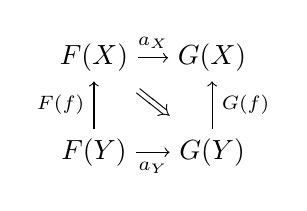
\begin{tikzpicture}
    \def\x{1.5}
    \def\y{-1.2}
    \node (A0_0) at (0*\x, 0*\y) {$F(X)$};
    \node (A0_1) at (1*\x, 0*\y) {$G(X)$};
    \node (A1_0) at (0*\x, 1*\y) {$F(Y)$};
    \node (A1_1) at (1*\x, 1*\y) {$G(Y)$};
    \path (A0_0) edge [->] node [auto] {$\scriptstyle{a_X}$} (A0_1);
    \path (A1_0) edge [->] node [auto,swap] {$\scriptstyle{a_Y}$} (A1_1);
    \path (A1_0) edge [->] node [auto] {$\scriptstyle{F(f)}$} (A0_0);
    \path (A1_1) edge [->] node [auto,swap] {$\scriptstyle{G(f)}$} (A0_1);
    \path (A0_0) -- (A1_1) 
      node [pos=0.5,sloped] {$\Longrightarrow$};
  \end{tikzpicture}
  \]
      such that
  \[
  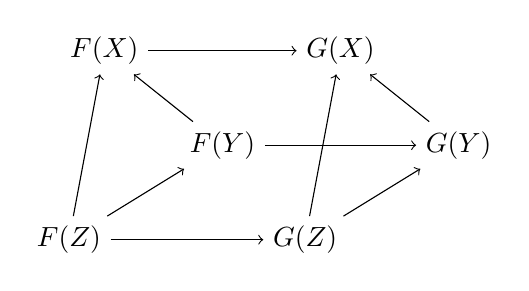
\begin{tikzpicture}
    \def\x{1.5}
    \def\y{-1.2}
    \node (A1_0) at (0.3*\x, 1*\y) {$F(X)$};
    \node (A1_2) at (2.3*\x, 1*\y) {$G(X)$};
    \node (A2_1) at (1.3*\x, 2*\y) {$F(Y)$};
    \node (A2_3) at (3.3*\x, 2*\y) {$G(Y)$};
    \node (A3_0) at (0*\x, 3*\y) {$F(Z)$};
    \node (A3_2) at (2*\x, 3*\y) {$G(Z)$};
    \path (A3_0) edge [->] node [auto] {$\scriptstyle{}$} (A2_1);
    \path (A3_0) edge [->] node [auto] {$\scriptstyle{}$} (A3_2);
    \path (A1_0) edge [->] node [auto] {$\scriptstyle{}$} (A1_2);
    \path (A3_2) edge [->] node [auto] {$\scriptstyle{}$} (A2_3);
    \path (A2_3) edge [->] node [auto] {$\scriptstyle{}$} (A1_2);
    \path (A3_2) edge [->] node [auto] {$\scriptstyle{}$} (A1_2);
    \path (A2_1) edge [->] node [auto] {$\scriptstyle{}$} (A1_0);
    \path (A2_1) edge [->] node [auto] {$\scriptstyle{}$} (A2_3);
    \path (A3_0) edge [->] node [auto] {$\scriptstyle{}$} (A1_0);
  \end{tikzpicture}
  \]
      is $2$-commutative, where the $2$-morphism on the triangular faces are the ones defined by the pseudofunctors $F$ and $G$, while the $2$-morphisms on the rectangular faces are the one defined before.
  \end{itemize}
\end{definition}

\begin{definition}
  Given $a, b\colon F → G$ where $F$ and $G$ are pseudofunctors, then a \emph{$2$-morphism of pseudofunctors\/} between $a$ and $b$ is denoted by $α\colon a ⇒ b$ and is the datum of:
  \begin{itemize}
    \item for every $X ∈ \Obj(ℭ)$, a $2$-morphism $α_X\colon a_X ⇒ b_X$ such that  for every $f\colon X → Y$, the diagram
  \[
  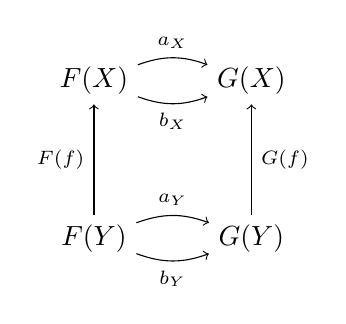
\begin{tikzpicture}
    \def\x{2}
    \def\y{-2}
    \node (A0_0) at (0*\x, 0*\y) {$F(X)$};
    \node (A0_1) at (1*\x, 0*\y) {$G(X)$};
    \node (A1_0) at (0*\x, 1*\y) {$F(Y)$};
    \node (A1_1) at (1*\x, 1*\y) {$G(Y)$};
    \path (A0_0) edge [->,bend left=20] node [auto] {$\scriptstyle{a_X}$} (A0_1);
    \path (A0_0) edge [->,bend right=20] node [auto,swap] {$\scriptstyle{b_X}$} (A0_1);
    \path (A1_0) edge [->,bend left=20] node [auto] {$\scriptstyle{a_Y}$} (A1_1);
    \path (A1_0) edge [->,bend right=20] node [auto,swap] {$\scriptstyle{b_Y}$} (A1_1);
    \path (A1_0) edge [->] node [auto] {$\scriptstyle{F(f)}$} (A0_0);
    \path (A1_1) edge [->] node [auto,swap] {$\scriptstyle{G(f)}$} (A0_1);
  \end{tikzpicture}
  \]
      is a $2$-commutative cylinder.
  \end{itemize}
\end{definition}

\nocite{*}
\bibliographystyle{amsalpha}
\bibliography{2009.01.12.Barbara.Fantechi.Algebraic.Stacks}


\end{document}
